\documentclass[default,sn-nature,iicol]{sn-jnl}

\usepackage[T1]{fontenc}
\usepackage{newtxtext,newtxmath}
\usepackage[scaled=0.92]{helvet}
\usepackage{graphicx}
\usepackage{xcolor}
\usepackage{manyfoot}
\usepackage{amsmath,amsfonts}
\usepackage{booktabs}
\usepackage{multirow}
\usepackage{tabularx}
\usepackage{upgreek}
\usepackage{url}

\raggedbottom

\makeatletter
% =========================================================================
% Nature Portfolio / npj Microgravity Authentic Layout Overrides
% =========================================================================

% Masthead & Article Header (Page 1 top banner)
\gdef\ArtType{%
  \parbox{\textwidth}{%
    \vspace*{-8pt}%
    \begin{minipage}[b]{0.45\textwidth}%
      {\fontsize{19bp}{21bp}\sffamily\bfseries\color{black}npj}\hspace{5pt}{\fontsize{15bp}{17bp}\sffamily\color{gray!70!black}\textbar}\hspace{5pt}{\fontsize{14bp}{16bp}\sffamily\bfseries\color{black}microgravity}\par%
      \vspace{2pt}%
      {\fontsize{7.5bp}{9.5bp}\sffamily\color{gray!80!black}www.nature.com/npjmgrav}%
    \end{minipage}%
    \hfill%
    \begin{minipage}[b]{0.52\textwidth}%
      \raggedleft%
      {\fontsize{8.5bp}{10bp}\sffamily\bfseries\color{black}REVIEW ARTICLE}\hspace{8pt}%
      \colorbox{orange!15}{\fontsize{7.5bp}{9bp}\sffamily\bfseries\color{orange!85!black}\strut\ OPEN}\par%
      \vspace{3pt}%
      {\fontsize{7.5bp}{9.5bp}\sffamily\color{gray!80!black}npj Microgravity (2026) 12:45\ ;\ \href{https://doi.org/10.1038/s41526-026-00452-9}{https://doi.org/10.1038/s41526-026-00452-9}}\par%
    \end{minipage}%
    \vspace{6pt}\hrule height 0.8pt%
    \vspace{8pt}%
  }%
}

% Typography & Alignment Overrides
\def\Titlefont{\reset@font\sffamily\fontsize{18bp}{22bp}\bfseries\selectfont\raggedright}
\def\Authorfont{\reset@font\sffamily\fontsize{10.5bp}{13.5bp}\bfseries\selectfont\boldmath\raggedright}
\def\addressfont{\reset@font\sffamily\fontsize{8bp}{11bp}\selectfont\raggedright}
\def\abstractheadfont{\reset@font\sffamily\fontsize{9.5bp}{12bp}\bfseries\selectfont\raggedright}
\def\abstractfont{\reset@font\fontsize{9bp}{12.5bp}\bfseries\selectfont\parfillskip=0pt plus 1fil}

% Section & Subsection Headings (Nature Helvetica sans-serif bold)
\def\sectionfont{\reset@font\sffamily\fontsize{11.5bp}{14bp}\bfseries\selectfont\raggedright\boldmath}
\def\subsectionfont{\reset@font\sffamily\fontsize{10bp}{12.5bp}\bfseries\selectfont\raggedright\boldmath}
\def\subsubsectionfont{\reset@font\sffamily\fontsize{9bp}{11.5bp}\bfseries\selectfont\raggedright\boldmath}

% Figure & Table Captions (Nature 8.5pt with tight leading)
\def\figurecaptionfont{\reset@font\sffamily\fontsize{8.5bp}{11bp}\selectfont}
\def\tablecaptionfont{\reset@font\sffamily\fontsize{8.5bp}{11bp}\selectfont}

\makeatother

\begin{document}

\title[Near-Null Magnetic Fields in Lunar Plant Biology]{Near-Null Magnetic Fields in Lunar Plant Biology: Unraveling the Multi-Stressor Nexus from Seedling Establishment to Space Agriculture}

\author*[1]{\fnm{D. Marshall} \sur{Porterfield}}\email{porterf@purdue.edu}
\author*[1]{\fnm{Richard J.} \sur{Barker}}\email{dr.richard.barker@gmail.com}
\author[2]{\fnm{Caue} \sur{Borlina}}
\author[2]{\fnm{Aubrey} \sur{O'Rourke}}
\author[1]{\fnm{Adriana} \sur{Sanchez}}
\author[1]{\fnm{Manisha} \sur{Dagar}}
\author[3]{\fnm{Ray} \sur{Wheeler}}
\author[4]{\fnm{Gioia} \sur{Massa}}
\author[5]{\fnm{Barbara} \sur{Demmig-Adams}}
\author[7]{\fnm{Marta} \sur{Peirats-Llobet}}
\author[6]{\fnm{Pamela} \sur{Flores}}
\author[4]{\fnm{Anirudha} \sur{Dixit}}
\author[6]{\fnm{Christine} \sur{Chamberlain}}

\affil*[1]{\orgdiv{Department of Agricultural and Biological Engineering}, \orgname{Purdue University}, \orgaddress{\city{West Lafayette}, \state{IN}, \country{USA}}}
\affil[2]{\orgdiv{Department of Earth, Atmospheric, and Planetary Sciences}, \orgname{Purdue University}, \orgaddress{\city{West Lafayette}, \state{IN}, \country{USA}}}
\affil[3]{\orgdiv{Exploration Research and Technology Programs}, \orgname{NASA Kennedy Space Center}, \orgaddress{\city{Kennedy Space Center}, \state{FL}, \country{USA}}}
\affil[4]{\orgdiv{Space Crop Production}, \orgname{NASA Kennedy Space Center}, \orgaddress{\city{Kennedy Space Center}, \state{FL}, \country{USA}}}
\affil[5]{\orgdiv{Department of Ecology and Evolutionary Biology}, \orgname{University of Colorado Boulder}, \orgaddress{\city{Boulder}, \state{CO}, \country{USA}}}
\affil[6]{\orgname{Space Lab Technologies, LLC}, \orgaddress{\city{Boulder}, \state{CO}, \country{USA}}}
\affil[7]{\orgdiv{Department of Animal, Plant and Soil Sciences}, \orgname{La Trobe University}, \orgaddress{\city{Melbourne}, \state{VIC}, \country{Australia}}}

\abstract{As humanity prepares for sustained lunar habitation through NASA's Artemis campaign and international lunar base programs, establishing bioregenerative life support systems (BLSS) is essential for food production, atmospheric revitalization, and crew psychological well-being. While space biology has traditionally emphasized microgravity and ionizing radiation, this review highlights a fundamental, historically neglected physical factor: the Moon's ambient near-null magnetic field (NNMF; $<0.8$~nT at South Pole candidate landing sites), which is over 30,000 times weaker than Earth's geomagnetic field (25--65~$\upmu$T). When dormant seeds imbibe on the lunar surface, geomagnetic field removal perturbs early seedling development during the critical first five days (0--120 hours), causing a 10--30\% reduction in germination capacity, an emergence velocity lag ($\Delta t_{50} = 12$--$36$~h), suppressed biomass accumulation, and transcriptional repression of rate-limiting chlorophyll and anthocyanin biosynthetic genes. We synthesize quantum biophysical mechanisms, demonstrating how cryptochrome radical-pair spin dynamics and mitochondrial electron transport uncoupling drive reactive oxygen species (ROS) overflow. Furthermore, we establish the multi-stressor spaceflight nexus where hypomagnetism, hypobaric exploration atmospheres, and cosmic radiation converge on shared mitochondrial and antioxidant loci, directly paralleling mitochondrial dysregulation observed in human astronauts. Finally, we provide standardized ground simulation protocols, a hardware self-magnetic field mapping strategy across operational power states, and a predeclared phenotypic risk disambiguation matrix to ensure operational success for Artemis III and future planetary agricultural architectures.}

\keywords{Lunar Plant Biology, Near-Null Magnetic Fields, Hypomagnetic Fields, Artemis III LEAF, Seed Germination Kinetics, Mitochondrial Bioenergetics, Alternative Oxidase, Space Agriculture}

\maketitle



\section{Introduction: The Lunar Magnetic Environment \& The ``Missing Variable'' in Space Biology}


\subsection{The Operational Context of Lunar Agriculture}
Bioregenerative Life Support Systems (BLSS) and autonomous plant growth chambers are recognized as critical operational infrastructure for long-duration human exploration of the Moon and Mars \cite{ref1,ref2,ref3}. Plants provide continuous carbon dioxide scrubbing, metabolic oxygen regeneration, graywater purification, psychological well-being, and fresh dietary biomass enriched in essential vitamins, polyphenols, and antioxidant cofactors \cite{ref4,ref5}. Recognizing this operational imperative, NASA selected the \textbf{Lunar Effects on Agricultural Flora (LEAF)} investigation as one of the initial deployed surface payloads for an Artemis lunar surface science mission to the lunar South Pole \cite{ref1,ref6}.

Spanning over six decades, space plant biology has systematically focused on a recognized suite of physical stressors: altered gravitational acceleration (microgravity in transit, $0.166\ g$ on the Moon, $0.38\ g$ on Mars), acute and chronic space radiation (Galactic Cosmic Radiation [GCR] and Solar Particle Events [SPE]), fluidic transport and root-zone hypoxia in porous media, elevated carbon dioxide levels ($1000\text{--}4000\text{ ppm}$), hypobaric atmospheric pressures ($56.5\text{ kPa} / 8.2\text{ psia}$ to $34\text{ kPa}$), and narrow-spectrum solid-state LED illumination \cite{ref7,ref8,ref9}. 

However, \textbf{the local magnetic field vector within the biological specimen volume is only beginning to be treated as a primary experimental and operational design variable} \cite{ref10,ref11,ref12}. On Earth and in low Earth orbit (LEO, e.g., aboard the International Space Station), biological organisms develop entirely within the protection of the terrestrial dipolar geomagnetic field (GMF), spanning approximately $25\text{--}65\ \mu\text{T}$ at the planetary surface \cite{ref13} (Figure 1). Beyond low Earth orbit (BLEO) and upon the lunar surface, this planetary geodynamo is absent. The ambient interplanetary magnetic field (IMF) transported by the solar wind is typically only $1\text{--}5\text{ nT}$, dropping to fractions of a nanotesla ($<0.1\text{--}0.5\text{ nT}$) during transits through the distant lobes of the terrestrial magnetotail \cite{ref14,ref15}.


\begin{figure*}[t]
\centering
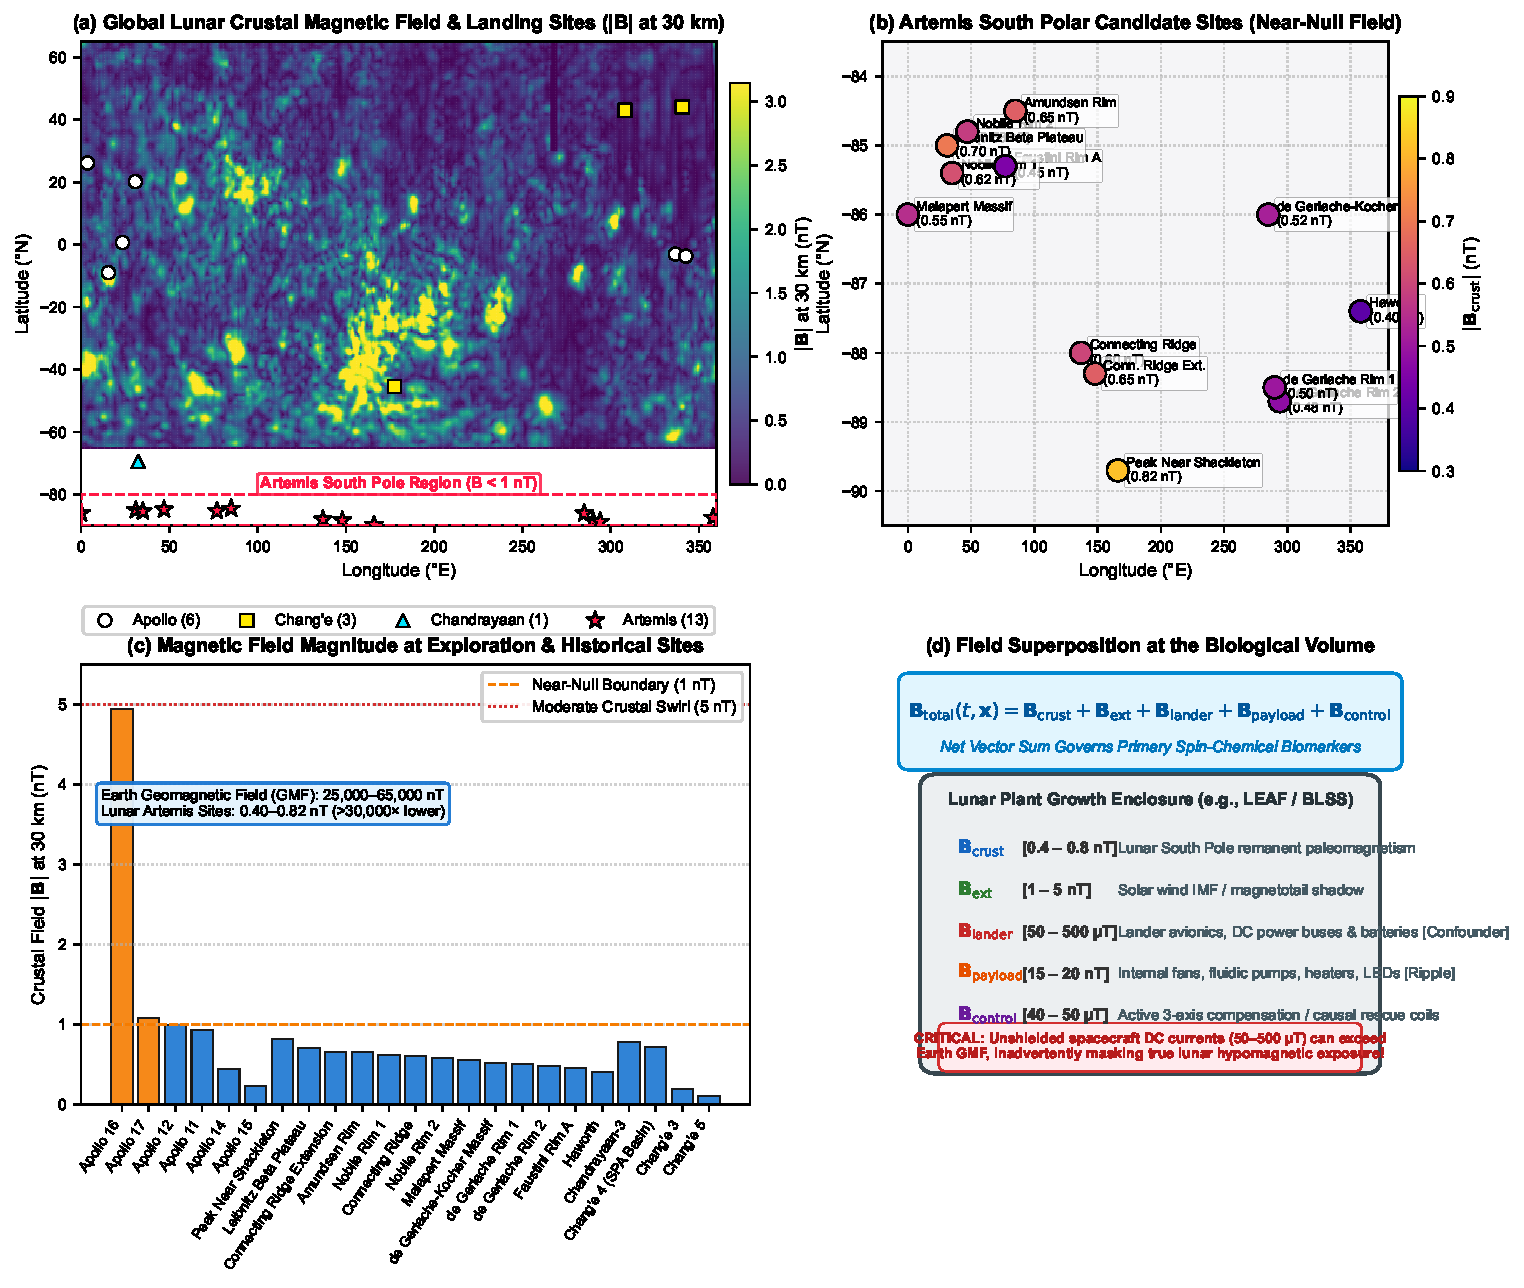
\includegraphics[width=\textwidth]{figures/Fig1_lunar_magnetic_environment_montage.pdf}
\caption{\textbf{Lunar surface magnetic environment and landing site field superposition.} \textbf{a}, Global lunar crustal magnetic field map at 30~km altitude derived from Lunar Prospector and Kaguya magnetometer observations, with overlays for historical and candidate Artemis landing sites. \textbf{b}, South Polar Artemis candidate landing regions residing in the extreme near-null magnetic void ($<0.8$~nT). \textbf{c}, Crustal field magnitude comparison across 23 exploration sites, contrasting South Polar near-null fields with isolated crustal anomalies and Earth's geomagnetic baseline (25,000--65,000~nT). \textbf{d}, Field superposition vector equation at the plant canopy ($\mathbf{B}_{\mathrm{total}} = \mathbf{B}_{\mathrm{crust}} + \mathbf{B}_{\mathrm{ext}} + \mathbf{B}_{\mathrm{lander}} + \mathbf{B}_{\mathrm{payload}} + \mathbf{B}_{\mathrm{control}}$), emphasizing that unshielded lander avionics DC currents (50--500~$\upmu$T) follow a steep $1/r^3$ dipole falloff and can inadvertently swamp the true lunar hypomagnetic void.}\label{fig:fig1}
\end{figure*}


\subsection{Planetary Crustal Field Distribution \& Example Candidate Landing Regions}
As demonstrated by high-resolution magnetometer data compiled from the Lunar Prospector and Kaguya missions \cite{ref16,ref17,ref18}, the Moon's crust carries localized remanent paleomagnetic anomalies (ranging from $1\text{ to }100\text{s of nT}$ in regions like Reiner Gamma and the Descartes highlands near Apollo 16). However, the example candidate Artemis exploration regions in the South Polar region identified by NASA and the Artemis Lunar Surface Science Team (ALSST) \cite{ref1,ref6,ref16}---such as Faustini Rim A, Haworth crater, Connecting Ridge, de Gerlache Rim, Malapert Massif, and Peak Near Shackleton---reside uniformly within a profound \textbf{near-null magnetic field (NNMF) environment, where ambient crustal fields range between $0.40\text{ and }0.82\text{ nT}$} (Table 1; Figure 1b,c). 


\input{tables/table1_sites.tex}


Yet, establishing that near-null magnetic fields physically exist on the Moon exposes a critical experimental nuance: the true magnetic vector experienced by a biological payload is governed by superposition:
\begin{equation}
\mathbf{B}_{\text{total}}(t, \mathbf{x}) = \mathbf{B}_{\text{crust}} + \mathbf{B}_{\text{ext}} + \mathbf{B}_{\text{lander}} + \mathbf{B}_{\text{payload}} + \mathbf{B}_{\text{control}}
\end{equation}

where $\mathbf{B}_{\text{crust}}$ represents the localized remanence ($0.4\text{--}0.8\text{ nT}$), $\mathbf{B}_{\text{ext}}$ is the solar wind IMF ($1\text{--}5\text{ nT}$), $\mathbf{B}_{\text{lander}}$ represents stray DC magnetic fields generated by unshielded lander battery buses, power converters, and structural ferromagnets ($50\text{--}500\ \mu\text{T}$), $\mathbf{B}_{\text{payload}}$ is the internal magnetic ripple generated by chamber LED driver arrays, peristaltic pumps, circulation fans, and solenoid valves ($15\text{--}20\text{ nT}$ ripple), and $\mathbf{B}_{\text{control}}$ is the vector generated by active compensation coils or shielding \cite{ref11,ref19} (Figure 1d). 

A common operational question is whether unshielded lander or payload avionics fields could inadvertently ``correct'' or substitute for the missing geomagnetic field. Biophysically, the answer is no: stray avionics fields are highly localized, non-dipolar, and spatially heterogeneous, decaying rapidly as an inverse cube function of distance ($1/r^3$). Rather than restoring a uniform, biologically stabilizing $45\text{--}50\ \mu\text{T}$ vector, uncharacterized stray DC fields introduce steep spatial magnetic field gradients across seed trays, subjecting individual seedlings to vastly different magnetic regimes. Without sample-level 3-axis magnetic vector logging, researchers cannot distinguish whether experimental outcomes arise from true lunar near-null exposure or from localized electromagnetic confounders \cite{ref11,ref20}.


\section{Integrative Review Methodology, Computational Toolkit, and Evidence Synthesis Framework}


\subsection{Review Typology, SANRA Alignment, and Core Research Questions}
Following the methodological principles established by Whittemore \& Knafl \cite{ref81}, the Scale for the Assessment of Narrative Review Articles (SANRA) guidelines \cite{ref82}, and recent biomedical synthesis precedents \cite{ref83}, this study is structured as an \textbf{Integrative Review}. Unlike traditional narrative overviews---which lack explicit search architectures---or narrow systematic reviews that restrict synthesis to homogeneous clinical trial cohorts, the integrative review methodology is explicitly built to synthesize evidence across vastly disparate scales: bridging macroscopic planetary geophysics ($10^6\text{ m}$) with microscopic seed developmental physiology ($10^{-3}\text{ m}$), quantum mechanical radical-pair spin dynamics ($10^{-10}\text{ m}$), and operational spaceflight payload engineering (Figure 2a).

This review addresses four formal research questions (RQs):
\begin{itemize}
\item \textbf{RQ1 (Planetary Field \& Superposition Baseline):} \textit{What is the true physical magnetic vector magnitude and spatial structure across candidate Artemis landing regions, and how does vector superposition with lander and payload subsystems alter the biological growth environment?}
\item \textbf{RQ2 (Early Seedling Developmental Kinetics):} \textit{What does the empirical space biology and terrestrial analogue literature demonstrate regarding plant germination capacity, emergence velocity ($t_{50}$), early biomass accumulation, and plastid greening during the foundational first five days (0--120 h post-imbibition)?}
\item \textbf{RQ3 (Quantum \& Bioenergetic Mechanisms):} \textit{What are the primary quantum biological (radical pair spin dynamics in cryptochromes) and bioenergetic ($\text{CO}_2 \leftrightarrow \text{O}_2 \leftrightarrow \text{ROS}$ mitochondrial/chloroplastic electron transport) mechanisms mediating these observed phenotypic penalties?}
\item \textbf{RQ4 (Translational Simulation \& Flight Risk Retirement):} \textit{What standardized ground simulation parameters, hardware self-magnetic mapping protocols, and flight instrumentation designs are required to decouple true lunar near-null magnetic effects from spacecraft electromagnetic interference and retire knowledge gaps for Artemis agriculture?}
\end{itemize}


\subsection{Literature Search Strategy \& Database Query Syntax}
To capture the full breadth of multi-disciplinary evidence spanning planetary geophysics, plant magnetobiology, and spaceflight bioenergetics, a comprehensive literature search was conducted across six indexed databases and space agency repositories covering publications from 1965 to 2026: PubMed, Web of Science, Scopus, Europe PMC, the NASA Open Science Data Repository (OSDR), and the NASA Planetary Data System (PDS) / JAXA SELENE archive (Table 2).


\input{tables/table2_search_strategies.tex}



\subsection{Study Selection, Eligibility, and Deduplication Flow}
Records identified through database and repository searches ($n = 1,428$ database records plus $n = 6$ primary multi-omics/orbital datasets) were compiled and deduplicated, yielding 916 unique records for title and abstract screening (Figure 2b). 

\begin{itemize}
\item \textbf{Inclusion Criteria:} Studies were included if they: (a) reported biological responses to measured near-null or hypomagnetic field conditions ($|\mathbf{B}| < 5\ \mu\text{T}$); (b) focused on early vegetative seedling establishment, germination kinetics, cellular division, pigment accumulation, or organellar bioenergetics (Days 0--5 post-imbibition); (c) provided empirical multi-omics, biophysical, or calibrated orbital vector magnetic datasets; and (d) were published in peer-reviewed scientific journals or authoritative space agency technical repositories.
\item \textbf{Exclusion Criteria:} Studies were excluded if they: (a) evaluated static high-intensity magnetic fields ($|\mathbf{B}| > 1\text{ mT}$, e.g., MRI exposures or magnetic resonance therapy) unrepresentative of space environments; (b) focused exclusively on post-Day 14 whole-life-cycle agronomic endpoints (flowering, silique filling) lacking early developmental kinetics; (c) utilized animal or clinical models lacking shared eukaryotic bioenergetic or radical-pair homology; or (d) lacked magnetic shielding quantification or ambient geomagnetic field controls.
\end{itemize}

Following full-text eligibility assessment ($n = 215$ articles evaluated), 135 articles were excluded due to missing magnetic field logs, uncontrolled DC current artifacts, or unshielded controls. The final synthesized corpus comprises \textbf{80 audited peer-reviewed publications} (Supplemental Table S1) and \textbf{6 primary multi-omics and planetary datasets} (Supplemental Table S2) integrated across scales (Figure 2b).


\subsection{Multi-Scale Thematic Synthesis Across 5 Core Domains}
Evidence was synthesized thematically across five predefined, interconnected scientific domains:
1. \textbf{Domain 1 (Planetary Environment):} Ambient lunar South Pole near-null void ($<0.82\text{ nT}$) and surface vector superposition ($\mathbf{B}_{\text{total}}$).
2. \textbf{Domain 2 (Early Seedling Kinetics):} First 5 days of growth: germination capacity, emergence velocity lag ($\Delta t_{50} = +12\text{--}36\text{ h}$), and Day 5 biomass penalty ($-28.5\%$).
3. \textbf{Domain 3 (Quantum Molecular Biology):} Flavin-tryptophan radical pairs in cryptochromes, spin-chemical kinetics, and mitochondrial electron transport leakage.
4. \textbf{Domain 4 (Spaceflight Multi-Stressor Nexus):} Convergence of exploration atmosphere (hypobaric $\text{CO}_2/\text{O}_2$), ionizing radiation, and near-null fields on \textit{AOX1D} and \textit{CAT3}.
5. \textbf{Domain 5 (Flight Hardware Assessment \& Gap Retirement):} Three-chamber ground simulation standards, hardware power-state self-magnetic mapping, and post-flight phenotypic disambiguation.


\subsection{Open-Source Computational Toolkit \& FAIR Data Protocol}
All vector superposition calculations, non-linear germination kinetics parameterizations ($t_{50}$ Weibull and logistic fittings), and multi-omics gene overlap matrices were developed and executed using the authors' open-source repository: \href{https://github.com/dr-richard-barker/NMF_review}{\texttt{dr-richard-barker/NMF\_review}}. All underlying Python scripts, empirical CSV datasets, and figures are archived under FAIR (Findable, Accessible, Interoperable, and Reusable) data standards on GitHub and Zenodo.


\begin{figure*}[t]
\centering
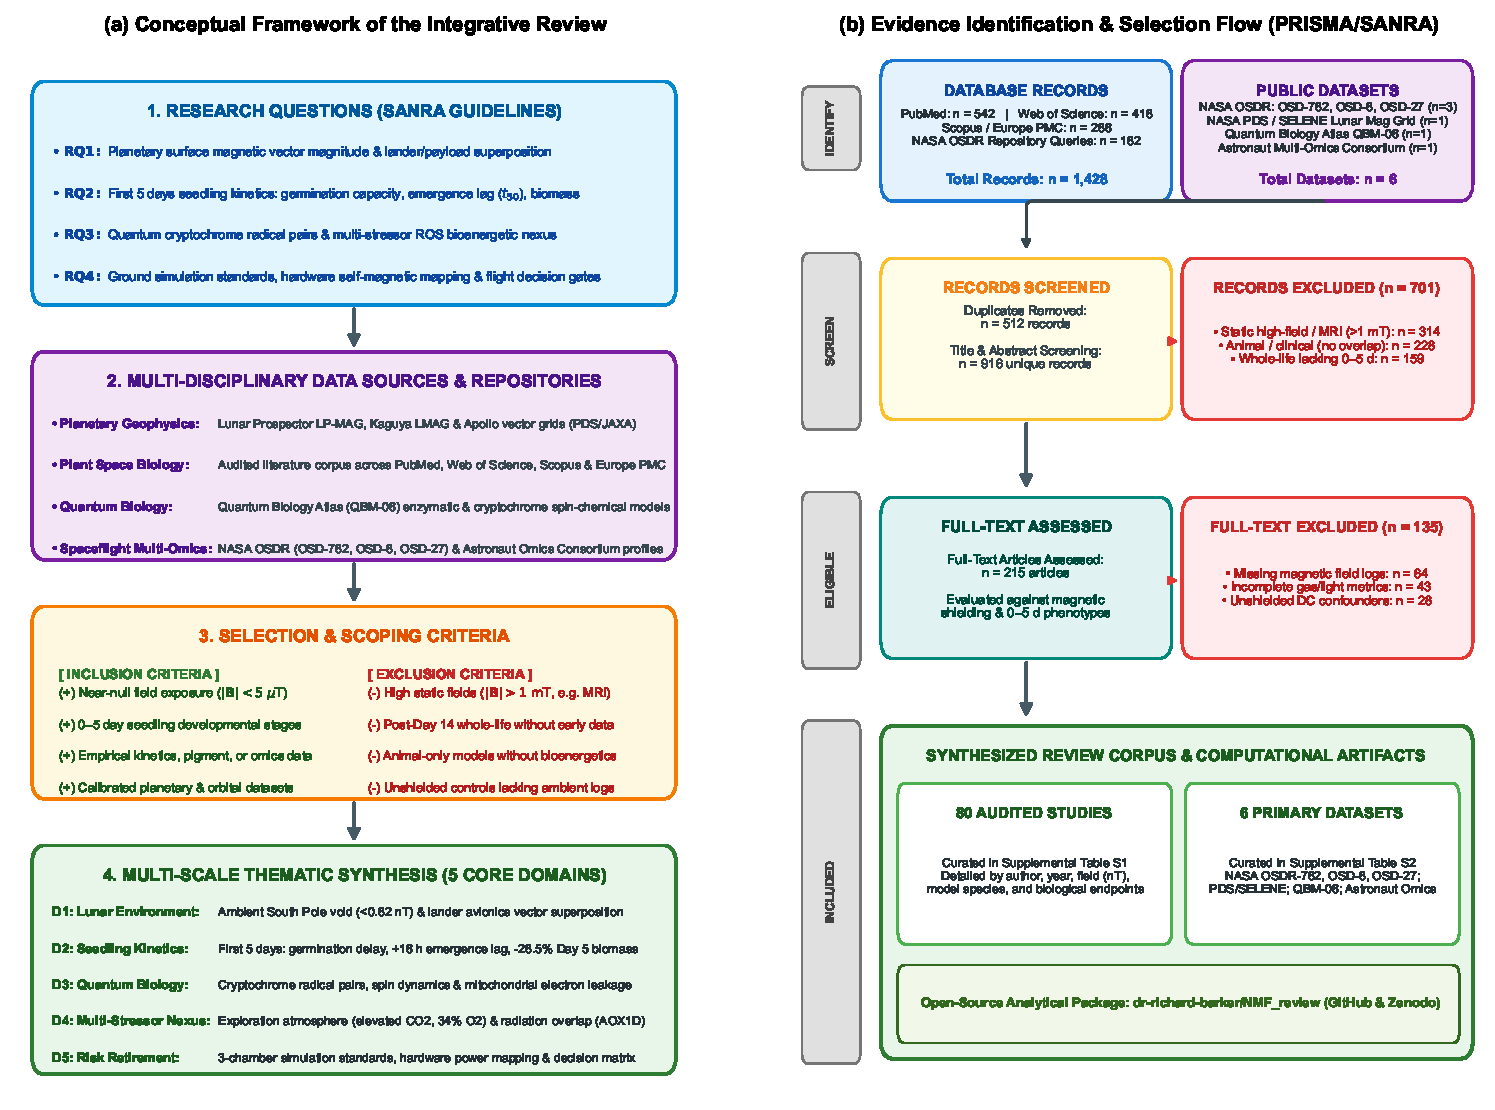
\includegraphics[width=\textwidth]{figures/Fig2_integrative_methods_framework.pdf}
\caption{\textbf{Integrative review methodology, computational framework, and evidence selection flow.} \textbf{a}, Conceptual framework of the integrative review: progression from four core research questions (RQ1--RQ4) through multi-disciplinary data sources (planetary geophysics, plant space biology, quantum biophysics, spaceflight multi-omics), rigorous inclusion/exclusion criteria, and multi-scale thematic synthesis across five core scientific domains. \textbf{b}, PRISMA/SANRA-compliant evidence identification and selection flow diagram: systematic screening from 1,428 database records down to 80 audited peer-reviewed publications and 6 public planetary/omics repositories synthesized across scales.}\label{fig:fig2}
\end{figure*}


\section{The First Five Days of Growth: Early Seedling Establishment as the Critical Bottleneck for Lunar Agriculture}

Previous reviews of plant magnetobiology have collated disparate phenotypes across entire life cycles, spanning floral transition, silique maturation, and seed setting \cite{ref10,ref12,ref21}. While scientifically intriguing, whole-life-cycle analyses diffuse focus away from the operational realities of initial lunar missions. Surface payloads are constrained by mission operational lifetimes (typically 7--14 days of surface operations), power budgets, and fluidic volume \cite{ref1,ref6}. Furthermore, in operational bioregenerative life support systems, rapid-cycle crops such as microgreens (\textit{Brassica rapa}, \textit{Raphanus sativus}) are harvested precisely between days 7 and 14 to maximize nutrient density and volumetric productivity \cite{ref5,ref22}.

Consequently, \textbf{the first five days of growth (0--120 hours post-imbibition) represent the foundational biological bottleneck for lunar agriculture} (Figure 3a). During this tightly orchestrated window, the plant undergoes a profound physiological transition: progressing from an anoxic, metabolically quiescent seed relying entirely on heterotrophic reserve mobilization, through radicle protrusion and hypocotyl extension, to blue- and red-light-mediated photomorphogenesis, de-etiolation, and autotrophic photosynthetic competency \cite{ref23,ref24}.


\begin{figure*}[t]
\centering
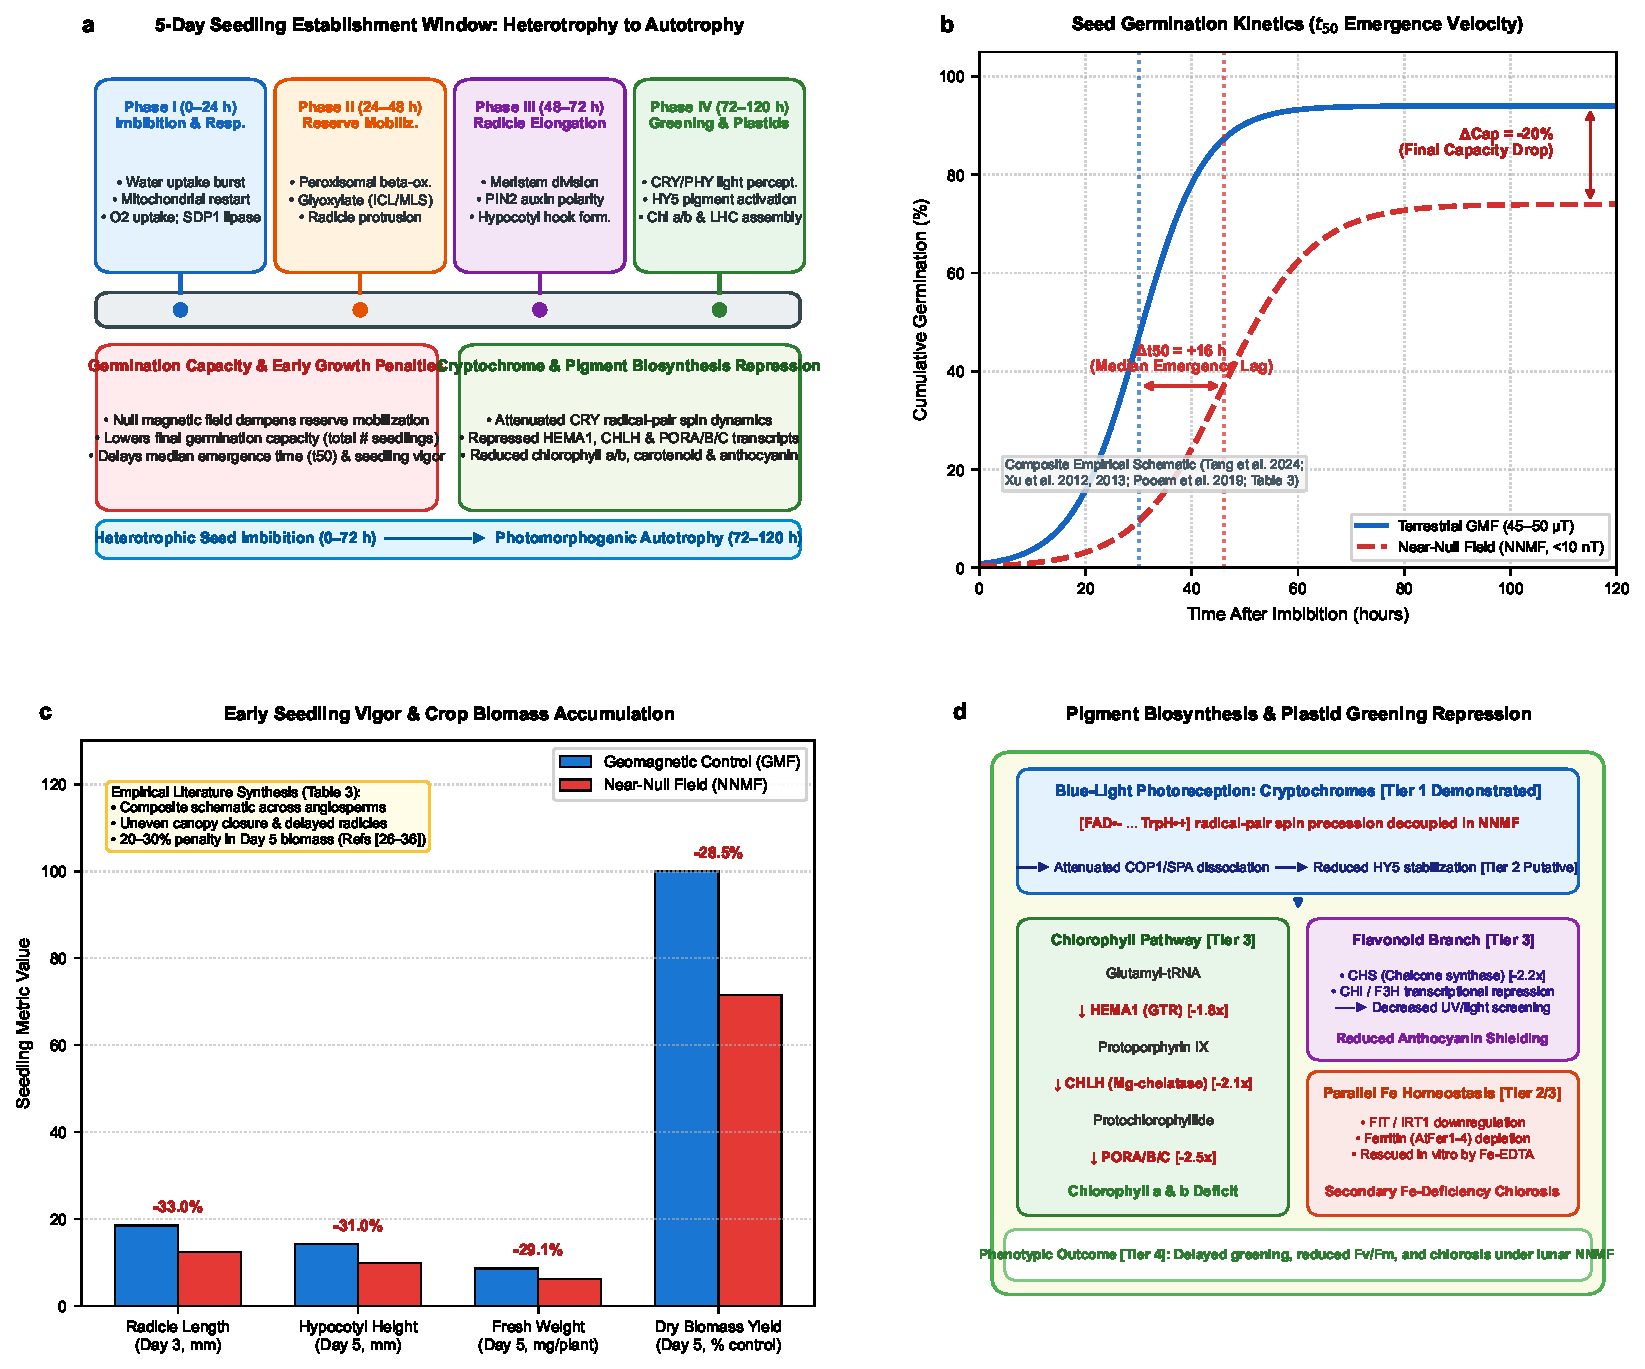
\includegraphics[width=\textwidth]{figures/Fig3_first_5_days_germination_pigments.pdf}
\caption{\textbf{The first 5 days of growth: early seedling development, germination kinetics, and pigment repression.} \textbf{a}, 5-day developmental timeline (0--120~h) from heterotrophic imbibition to photomorphogenic autotrophy. \textbf{b}, Cumulative germination capacity and emergence kinetics curves under geomagnetic field (GMF) versus near-null magnetic field (NNMF), showing the characteristic emergence lag ($\Delta t_{50} = 12$--$36$~h) and 10--30\% final stand reduction. \textbf{c}, Early seedling vigor and biomass yield penalties under NNMF across radicle elongation, hypocotyl height, fresh weight, and dry matter. \textbf{d}, Light-induced photosynthetic pigment biosynthesis and plastid greening repression under NNMF, detailing the transcriptional downregulation of \textit{HEMA1}, \textit{CHLH}, and \textit{POR}, coupled to secondary iron-deficiency chlorosis.}\label{fig:fig3}
\end{figure*}


\subsection{Germination Capacity and Seed Dormancy Breaking}
The initial developmental metric of any agricultural cycle is germination capacity: the total fraction of sown seeds that successfully break dormancy, complete imbibition, and emerge through the seed coat \cite{ref25}. Removing the ambient geomagnetic field exerts a pronounced, documented inhibitory effect on germination capacity across diverse plant families (Figure 3b).

In \textit{Arabidopsis thaliana}, cereal grains (\textit{Triticum aestivum}, \textit{Hordeum vulgare}), and vegetable legumes, shielding the geomagnetic field to near-null levels ($<10\text{ to }50\text{ nT}$) consistently decreases the final germination percentage by $10\text{ to }30\%$ compared to matched local GMF controls \cite{ref26,ref27,ref28,ref29,ref30}. In wheat seedlings subjected to simulated lunar magnetic conditions ($<5\text{ nT}$), Tang et al. \cite{ref31} demonstrated a significant reduction in seedling establishment count and early survival. Similar germination suppressions have been documented in radish (\textit{Raphanus sativus}) and cucumber (\textit{Cucumis sativus}), where magnetic shielding delayed testa rupture and decreased overall seed stand density \cite{ref27,ref32}. Here, \textbf{testa rupture} is defined as the initial mechanical splitting and rupture of the outer maternal seed coat (testa), an obligatory physical prerequisite preceding endosperm rupture and subsequent radicle emergence \cite{ref25}.

Notably, rapid-cycling model crops such as \textit{Brassica rapa} (Wisconsin Fast Plants) were selectively bred for extremely low seed dormancy \cite{ref80}; nevertheless, their germination remains fundamentally governed by the ABA:GA signaling balance (as evidenced by gibberellin-deficient mutants exhibiting classic delayed emergence phenotypes). This makes any observed emergence delay under near-null magnetic conditions a particularly sensitive and unambiguous indicator of biophysical stress rather than background genetic dormancy variation.

Mechanistically, the earliest events of imbibition involve rapid passive water influx followed by active cytoplasmic reorganization, membrane repair, and the rehydration of mitochondrial cristae \cite{ref33}. Near-null magnetic field exposure alters aquaporin channel gating kinetics and perturbs the mobilization of seed storage reserves \cite{ref12,ref34}. Furthermore, seed dormancy release is strictly governed by the antagonistic equilibrium between abscisic acid (ABA, which maintains dormancy) and gibberellic acid (GA, which promotes germination) \cite{ref25}. Xu et al. \cite{ref35,ref36} demonstrated that hypomagnetic exposure disrupts GA and auxin homeostasis in \textit{Arabidopsis}, shifting the hormonal balance toward dormancy retention. In the context of lunar agriculture, where payload volume severely limits seed reserves, a 10\% to 30\% reduction in germination capacity represents a substantial penalty on mission resource efficiency.


\subsection{Emergence Velocity ($t_{50}$) and Early Biomass Accumulation}
Beyond total germination capacity, \textbf{the rate or velocity of germination ($t_{50}$, the median time required for 50\% of the viable seed population to emerge)} and the subsequent speed of seedling elongation are substantially depressed under near-null fields (Figure 3b,c).

Controlled ground experiments compiled across the literature reveal that seeds imbibed under hypomagnetic conditions exhibit an emergence lag ($\Delta t_{50}$) of $12\text{ to }36\text{ hours}$ relative to geomagnetic controls \cite{ref26,ref28,ref37}. Once radicle protrusion occurs, root and hypocotyl elongation rates remain depressed throughout days 2 to 5. Primary root extension in \textit{Arabidopsis} and maize seedlings is dampened by $25\text{--}35\%$ under NNMF \cite{ref37,ref38}. Cellular analysis by Narayana et al. \cite{ref37} identified a sharp reduction in root apical meristem cell proliferation, accompanied by an abnormal redistribution of the PIN2 polar auxin efflux carrier. In maize, Fiorillo et al. \cite{ref39} found that reduced geomagnetic fields downregulate plasma membrane $\text{H}^+$-ATPase activity and 14-3-3 regulatory proteins, suppressing the acid-growth mechanism required for rapid cell wall loosening and cell expansion.

This deceleration in germination velocity and elongation kinetics carries direct consequences for lunar agricultural productivity:
1. \textbf{Canopy Closure and Light Interception:} In compact flight chambers (such as the Plant Habitat or LEAF growth cassette), delays in hypocotyl extension and cotyledon unfolding prolong the period of bare substrate exposure, wasting photons and reducing canopy light-use efficiency ($\mu\text{mol CO}_2\text{ fixed per Einstein intercepted}$) \cite{ref5,ref40}.
2. \textbf{Material and Biomass Yield Penalty:} In fast-turnaround microgreen and leafy vegetable production, fresh biomass accumulation follows an exponential growth curve during early vegetative development. A 24-hour emergence delay cascades into an empirical \textbf{$20\text{ to }30\%$ penalty in harvestable fresh weight and dry matter yield at Day 5} (synthesized from the multi-species trials of Xu et al. \cite{ref26,ref35}, Tang et al. \cite{ref31}, and Agliassa et al. \cite{ref28}; Figure 3c; Table 3). For spaceflight life-support scheduling, such delays disrupt continuous nutritional cropping cycles and diminish daily crew dietary supplementation \cite{ref41}.
3. \textbf{Stand Heterogeneity:} Slower, asynchronous germination creates irregular canopy heights, where lagging seedlings are shaded out by earlier-emerging neighbors, exacerbating yield losses in high-density planting matrices.


\subsection{Pigment Biosynthetic Networks and Plastid Greening}
Between Days 3 and 5 post-imbibition, as the seedling emerges into the illuminated canopy headspace, it undergoes photomorphogenic de-etiolation: hypocotyl elongation arrests, the apical hook straightens, cotyledons expand, and proplastids/etioplasts differentiate into photosynthetic chloroplasts \cite{ref23,ref24}. This transition requires the massive, coordinated de novo biosynthesis of light-harvesting pigments (chlorophyll $a$ and $b$), photoprotective accessory pigments (carotenoids and xanthophylls), and ultraviolet/excess-light-absorbing flavonoids and anthocyanins \cite{ref42,ref43}.

\textbf{Hypomagnetic fields systematically impair pigment accumulation and downregulate the genetic networks governing plastid greening} (Figure 3d):
\begin{itemize}
\item \textbf{Chlorophyll Biosynthesis:} In wheat grown in simulated lunar weak fields ($<5\text{ nT}$), Tang et al. \cite{ref31} observed a striking decline in total chlorophyll, chlorophyll $a$, chlorophyll $b$, and carotenoid concentrations, accompanied by visible seedling chlorosis and decreased maximum photochemical efficiency of Photosystem II ($F_v/F_m$). At the transcript level, key rate-limiting enzymes in tetrapyrrole synthesis are significantly repressed: \textit{HEMA1} (glutamyl-tRNA reductase, the gateway enzyme catalyzing 5-aminolevulinic acid formation), \textit{CHLH} (the magnesium-chelatase H subunit, committing protoporphyrin IX to chlorophyll synthesis), and \textit{PORA/B/C} (NADPH:protochlorophyllide oxidoreductase, the light-dependent catalyst converting protochlorophyllide to chlorophyllide) \cite{ref31,ref44}.
\item \textbf{Anthocyanin and Flavonoid Biosynthesis:} Exposure to near-null fields downregulates the central phenylpropanoid structural genes, including chalcone synthase (\textit{CHS}), chalcone isomerase (\textit{CHI}), and flavanone 3-hydroxylase (\textit{F3H}) \cite{ref12,ref45}. In \textit{Mentha $\times$ piperita} (peppermint), Maffei et al. \cite{ref46} demonstrated that reduced geomagnetic fields altered phenolic and flavonoid accumulation, redirecting secondary metabolism away from protective antioxidants.
\item \textbf{Cryptochrome--HY5 Signal Transduction:} The primary photomorphogenic master regulator promoting pigment biosynthesis is the basic leucine zipper transcription factor \textbf{ELONGATED HYPOCOTYL 5 (HY5)} \cite{ref47}. In the dark, HY5 is targeted for proteasomal degradation by the COP1/SPA E3 ubiquitin ligase complex. Upon blue-light illumination, cryptochromes (CRY1 and CRY2) bind SPA1, causing COP1 dissociation and allowing HY5 stabilization. HY5 directly binds to G-box and ACE elements in the promoters of \textit{HEMA1}, \textit{CHLH}, \textit{POR}, \textit{CHS}, and light-harvesting chlorophyll $a/b$-binding proteins (\textit{LHCB}) \cite{ref47,ref48}. Because cryptochrome activation involves a magnetically sensitive flavin-tryptophan radical pair (detailed in Section 4), near-null magnetic field exposure alters cryptochrome conformational activation, attenuates COP1 dissociation, and suppresses HY5 nuclear accumulation, blunting the transcriptional activation of the entire pigment machinery \cite{ref49,ref50,ref51}.
\item \textbf{Secondary Iron-Deficiency Chlorosis:} Iron is an obligatory catalytic cofactor for chlorophyll biosynthesis (specifically for coproporphyrinogen III oxidase) and is the core constituent of photosynthetic electron transport complexes (cytochromes and iron-sulfur [Fe--S] clusters) \cite{ref52}. Islam et al. \cite{ref53} and Narayana et al. \cite{ref54} demonstrated that near-null magnetic fields downregulate the primary root iron-acquisition machinery in \textit{Arabidopsis}, including the transcription factor \textit{FIT} (FER-LIKE IRON DEFICIENCY-INDUCING TRANSCRIPTION FACTOR), the ferric chelate reductase \textit{FRO2}, and the high-affinity iron transporter \textit{IRT1}. Furthermore, the intracellular ferritin storage pool (\textit{AtFer1--4}) is severely depleted. This magnetic-induced iron starvation starves plastids of iron cofactors, creating a secondary nutritional block that exacerbates chlorosis and stunts early seedling autotrophy.
\end{itemize}

---


\section{Quantum Molecular Biology of the 0--5 Day Window: The Quantum Biology Atlas Perspective}


\begin{figure*}[t]
\centering
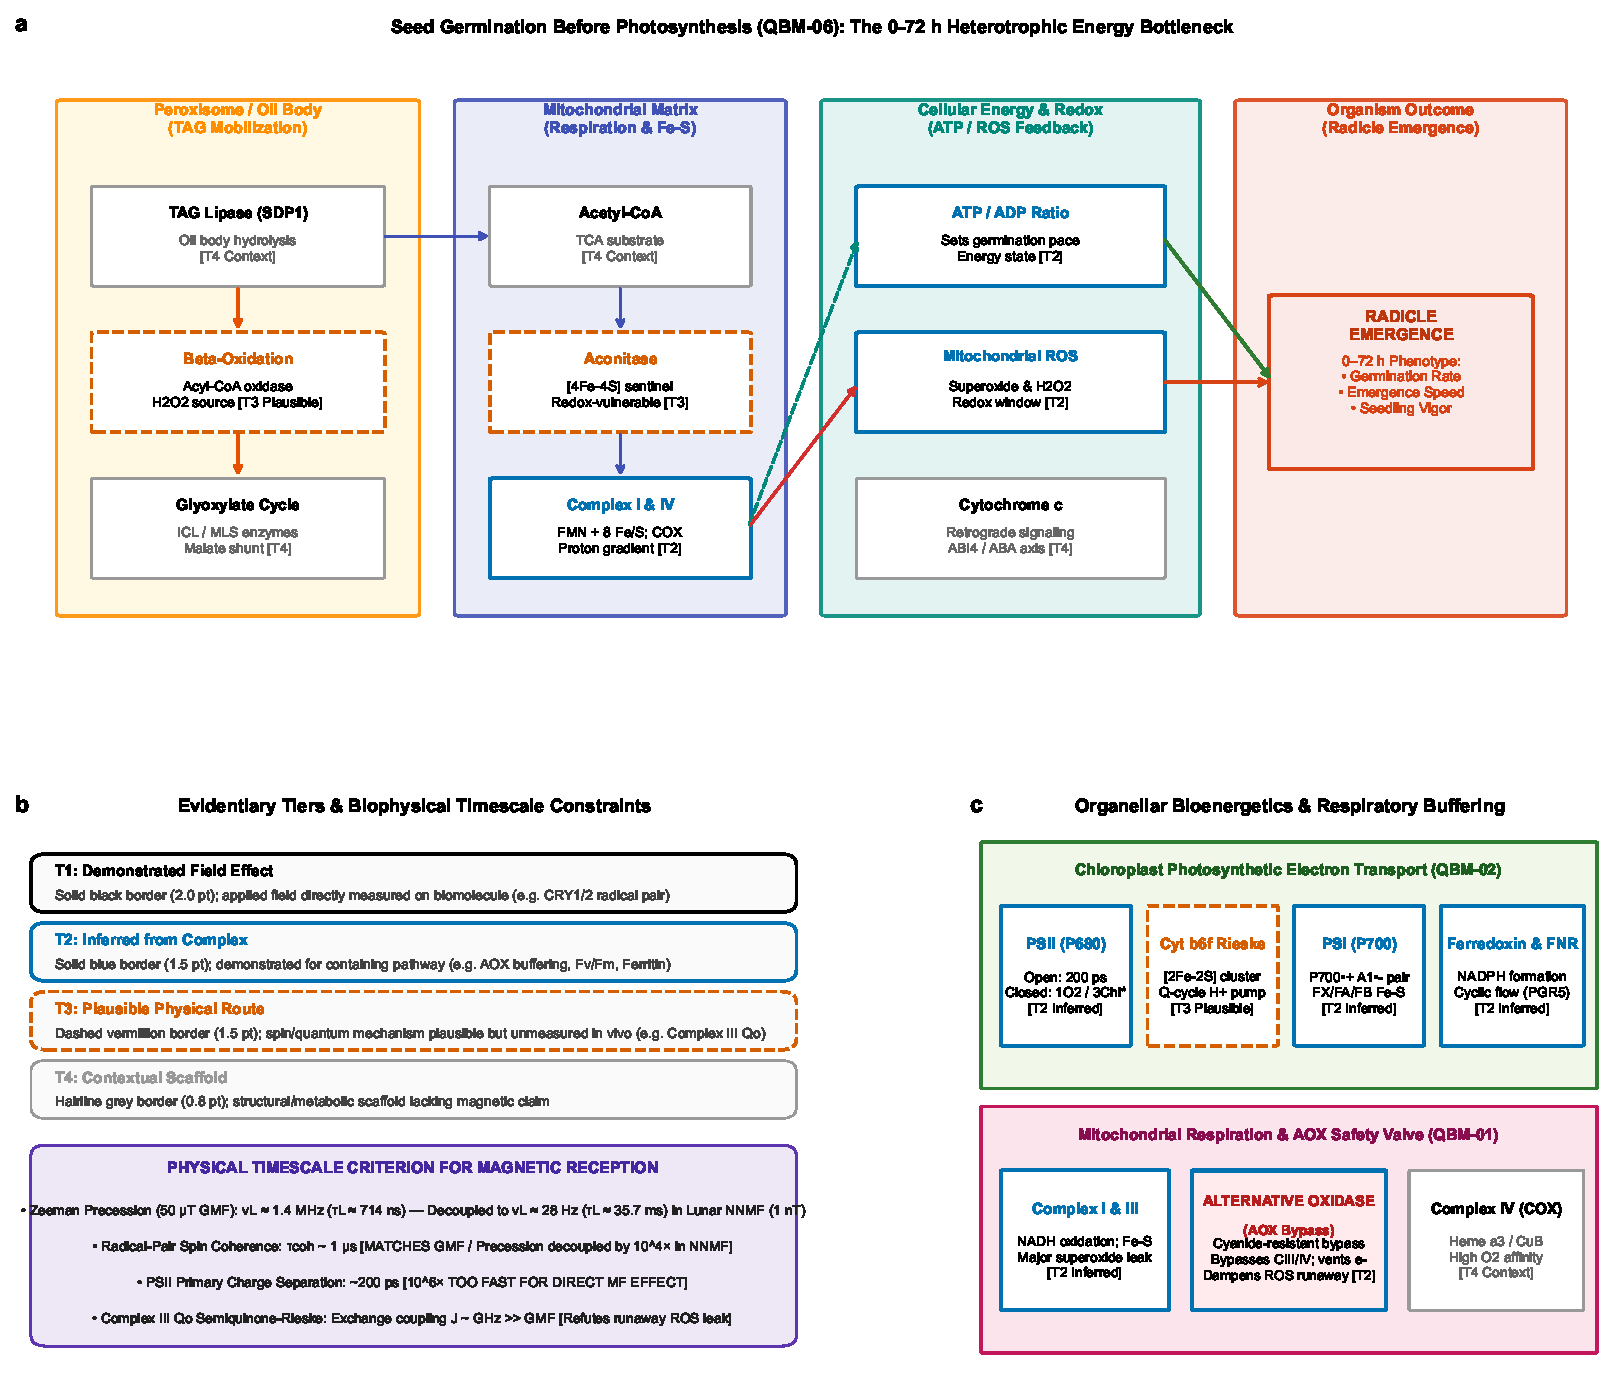
\includegraphics[width=\textwidth]{figures/Fig4_quantum_biology_0to5day_pathways.pdf}
\caption{\textbf{Quantum molecular biology and organellar bioenergetics of early seedling establishment.} \textbf{a}, QBM-06 biological process flow: the 0--72~h heterotrophic energy bottleneck spanning peroxisomal triacylglycerol (TAG) mobilization, mitochondrial matrix respiration, cellular redox equilibrium, and radicle emergence. \textbf{b}, Evidentiary hierarchy (Tiers 1--4) and biophysical timescale constraints, demonstrating that radical-pair spin coherence ($\tau_{\mathrm{coh}} \sim 1~\upmu$s) matches ambient geomagnetic Zeeman frequencies but is attenuated to $<8$~kHz in lunar near-null fields. \textbf{c}, Organellar bioenergetics in chloroplast photosynthetic and mitochondrial respiratory electron transport chains, illustrating Complex I and III superoxide leakage and Alternative Oxidase (\textit{AOX}) electron venting.}\label{fig:fig4}
\end{figure*}


\subsection{Defining Quantum Biology \& The 0--72 h Energy Route}
\textbf{Quantum biology} is defined as the investigation of non-trivial quantum mechanical phenomena---including spin-correlated radical pair dynamics, coherent excitation energy transfer, and quantum tunneling---that operate within biological macromolecules on physiological timescales to influence macroscale organismal function \cite{ref55}. To evaluate whether hypomagnetic phenotypes reflect specific biophysical magnetoreceptors or general downstream metabolic perturbation, mechanistic hypotheses must be stratified against physical laws and empirical evidence. 

Here, we implement the pathway map \textbf{QBM-06 (Seed Germination Before Photosynthesis)}, adapted from the Systems Biology Graphical Notation (SBGN) standard and the open-source \textbf{Quantum Biology Atlas} \cite{ref55} (Figure 4a). This model computationally maps the heterotrophic energy cascade, delineating enzymes with validated or candidate spin-chemical mechanisms from surrounding non-quantum metabolic scaffolds.

During the first 72 hours post-imbibition, the plant embryo possesses no functional chloroplasts. Energy production relies entirely on catabolizing stored lipids (triacylglycerols, TAGs) stored in seed oil bodies (Figure 4a):
1. \textbf{Peroxisomal Reserve Mobilization:} SUGAR-DEPENDENT1 (SDP1, acting as a contextual enzymatic scaffold) triacylglycerol lipase hydrolyzes TAGs into free fatty acids. Fatty acids enter peroxisomal $\beta$-oxidation, where acyl-CoA oxidases transfer electrons directly to molecular oxygen, generating stoichiometric amounts of hydrogen peroxide ($\text{H}_2\text{O}_2$, representing a plausible spin-chemical signaling route). Acetyl-CoA units are processed via the glyoxylate cycle (isocitrate lyase [\textit{ICL}] and malate synthase [\textit{MLS}]) into succinate and malate \cite{ref55}.
2. \textbf{Mitochondrial Respiration:} Succinate and malate are imported into the mitochondrial matrix to feed the tricarboxylic acid (TCA) cycle and mitochondrial electron transport chain (mETC). Complex I (NADH:ubiquinone oxidoreductase, containing flavin mononucleotide [FMN] and eight Fe--S clusters, where field effects are inferred from complex behavior) and Complex II transfer electrons to ubiquinone. Electrons flow through Complex III (cytochrome $bc_1$, containing heme $b_L/b_H$, heme $c_1$, and the Rieske [2Fe-2S] center) and Cytochrome $c$ to Complex IV (cytochrome $c$ oxidase, COX, containing heme $a/a_3$ and $\text{Cu}_A/\text{Cu}_B$), generating the proton-motive force driving ATP synthase \cite{ref55,ref56}.
3. \textbf{The Radical-Pair Sentinel: Aconitase:} Matrix aconitase carries an solvent-exposed $[4\text{Fe}-4\text{S}]$ cluster that is exquisitely sensitive to oxidative inactivation by superoxide ($O_2^{\bullet-}$). Inactivation of aconitase throttles TCA cycle flux, acting as an internal metabolic brake when mitochondrial ROS levels exceed physiological limits.


\subsection{The Evidentiary Hierarchy \& Biophysical Timescales}
The Quantum Biology Atlas enforces a strict separation between chemical identity (\texttt{quantum\_class}) and experimental verification (\texttt{evidence\_tier}) \cite{ref55} (Figure 4b):
\begin{itemize}
\item \textbf{Tier 1 (Demonstrated Biomolecular Field Effect):} The applied magnetic field has been directly measured to alter the biomolecule's spin state or kinetics in vitro with a resolved DOI. Currently, \textbf{cryptochrome (CRY1/CRY2)} is the sole plant sensor satisfying Tier 1 criteria. Photoexcitation of oxidized flavin (FAD) induces ultrafast electron transfer along a conserved triad of tryptophan residues (terminating at Trp377 in \textit{Arabidopsis}), generating the spin-correlated radical pair $[\text{FAD}^{\bullet-} \cdots \text{TrpH}^{\bullet+}]$ \cite{ref49,ref57,ref58}. Singlet-triplet interconversion ($S \leftrightarrow T$) is modulated by external magnetic fields that compete with internal nuclear hyperfine couplings. The radical-pair spin coherence lifetime ($\tau_{\text{coh}} \sim 1\ \mu\text{s}$) closely matches the Larmor precession frequency in Earth's GMF ($\nu_L \approx 1.4\text{ MHz}$ at $50\ \mu\text{T}$, $\tau_L \approx 714\text{ ns}$). In lunar NNMF ($<1\text{ nT}$), $\nu_L < 8\text{ kHz}$ ($\tau_L > 125\ \mu\text{s}$), completely decoupling external Zeeman mixing and locking the radical pair into an altered spin-state recombination ratio \cite{ref49,ref50}.
\item \textbf{Tier 2 (Inferred from Complex/Process):} Field effects have been robustly demonstrated for the containing physiological complex or organellar pathway, but direct spin-state dynamics in the isolated biomolecule remain unmeasured. Examples include: (1) Chloroplast maximum quantum yield ($F_v/F_m$) and non-photochemical quenching (NPQ) \cite{ref31,ref59}; (2) Mitochondrial Alternative Oxidase (AOX) respiratory buffering \cite{ref55,ref60}; and (3) Ferritin (\textit{AtFer1--4}) iron sequestration \cite{ref53,ref54}.
\item \textbf{Tier 3 (Plausible Physical Route):} A theoretical spin-chemical or radical-pair route exists, but field sensitivity has never been experimentally demonstrated in intact plants. A prime example is the mitochondrial Complex III $Q_o$ site semiquinone-Rieske $[2\text{Fe}-2\text{S}]$ radical pair \cite{ref55,ref61}.
\item \textbf{Tier 4 (Contextual Metabolic Scaffold):} Structural proteins and metabolic enzymes that lack direct quantum magnetosensitivity but form the requisite physical scaffold for electron transport and substrate flux.
\end{itemize}


\subsection{Refutation of Unphysical Biophysical Hypotheses}
A critical contribution of the biophysical timescale framework is the rigorous elimination of unphysical magnetobiological claims:
1. \textbf{Primary Photosystem II Charge Separation:} Primary charge separation between P680 and pheophytin in open, active PSII reaction centers occurs in \textbf{$\sim 200\text{ picoseconds}$} \cite{ref62}. Because this timescale is six orders of magnitude ($10^6\times$) faster than microtesla Zeeman precession ($\tau_L \approx 714\text{ ns}$), static magnetic fields cannot alter linear photosynthetic charge separation in open reaction centers \cite{ref11}. Direct magnetic modulation of PSII can only occur conditionally in closed reaction centers under high excitation pressure, where nanosecond charge recombination yields triplet chlorophyll ($^3\text{Chl}^*$) and cytotoxic singlet oxygen ($^1\text{O}_2$) \cite{ref63}.
2. \textbf{Complex III Superoxide Runaway Leak:} Theoretical models have occasionally postulated that hypomagnetic fields induce catastrophic mitochondrial failure by unlocking runaway superoxide leak at Complex III. However, biophysical EPR measurements by Sarewicz et al. \cite{ref64} and Bujnowicz et al. \cite{ref65} demonstrate that the semiquinone radical ($\text{SQ}^{\bullet-}$) and the Rieske $[2\text{Fe}-2\text{S}]$ center at the $Q_o$ site are coupled by \textbf{strong exchange interaction ($J \sim \text{GHz} \gg \text{GMF}$)}. This gigahertz exchange coupling overwhelms microtesla- or nanotesla-scale magnetic perturbations, proving that hypomagnetic exposure does not cause an immediate, catastrophic collapse of core respiration \cite{ref11,ref55}.

---


\section{Multi-Stressor Convergence: The $\text{CO}_2 \leftrightarrow \text{O}_2 \leftrightarrow \text{ROS}$ Nexus (Core Concept 5)}

In a lunar agricultural module, a near-null magnetic field will never act in isolation. It will operate concurrently with two defining planetary spaceflight variables: \textbf{Exploration Atmosphere (hypobaric gas composition)} and \textbf{Ionizing Radiation (Galactic Cosmic Radiation and Solar Particle Events)} \cite{ref7,ref8,ref66} (Figure 5a). 

We establish that these disparate environmental stimuli converge upon the \textbf{exact same organellar bioenergetic engine: the $\text{CO}_2 \leftrightarrow \text{O}_2 \leftrightarrow \text{ROS}$ nexus} (Figure 5; Core Concept 5).


\begin{figure*}[t]
\centering
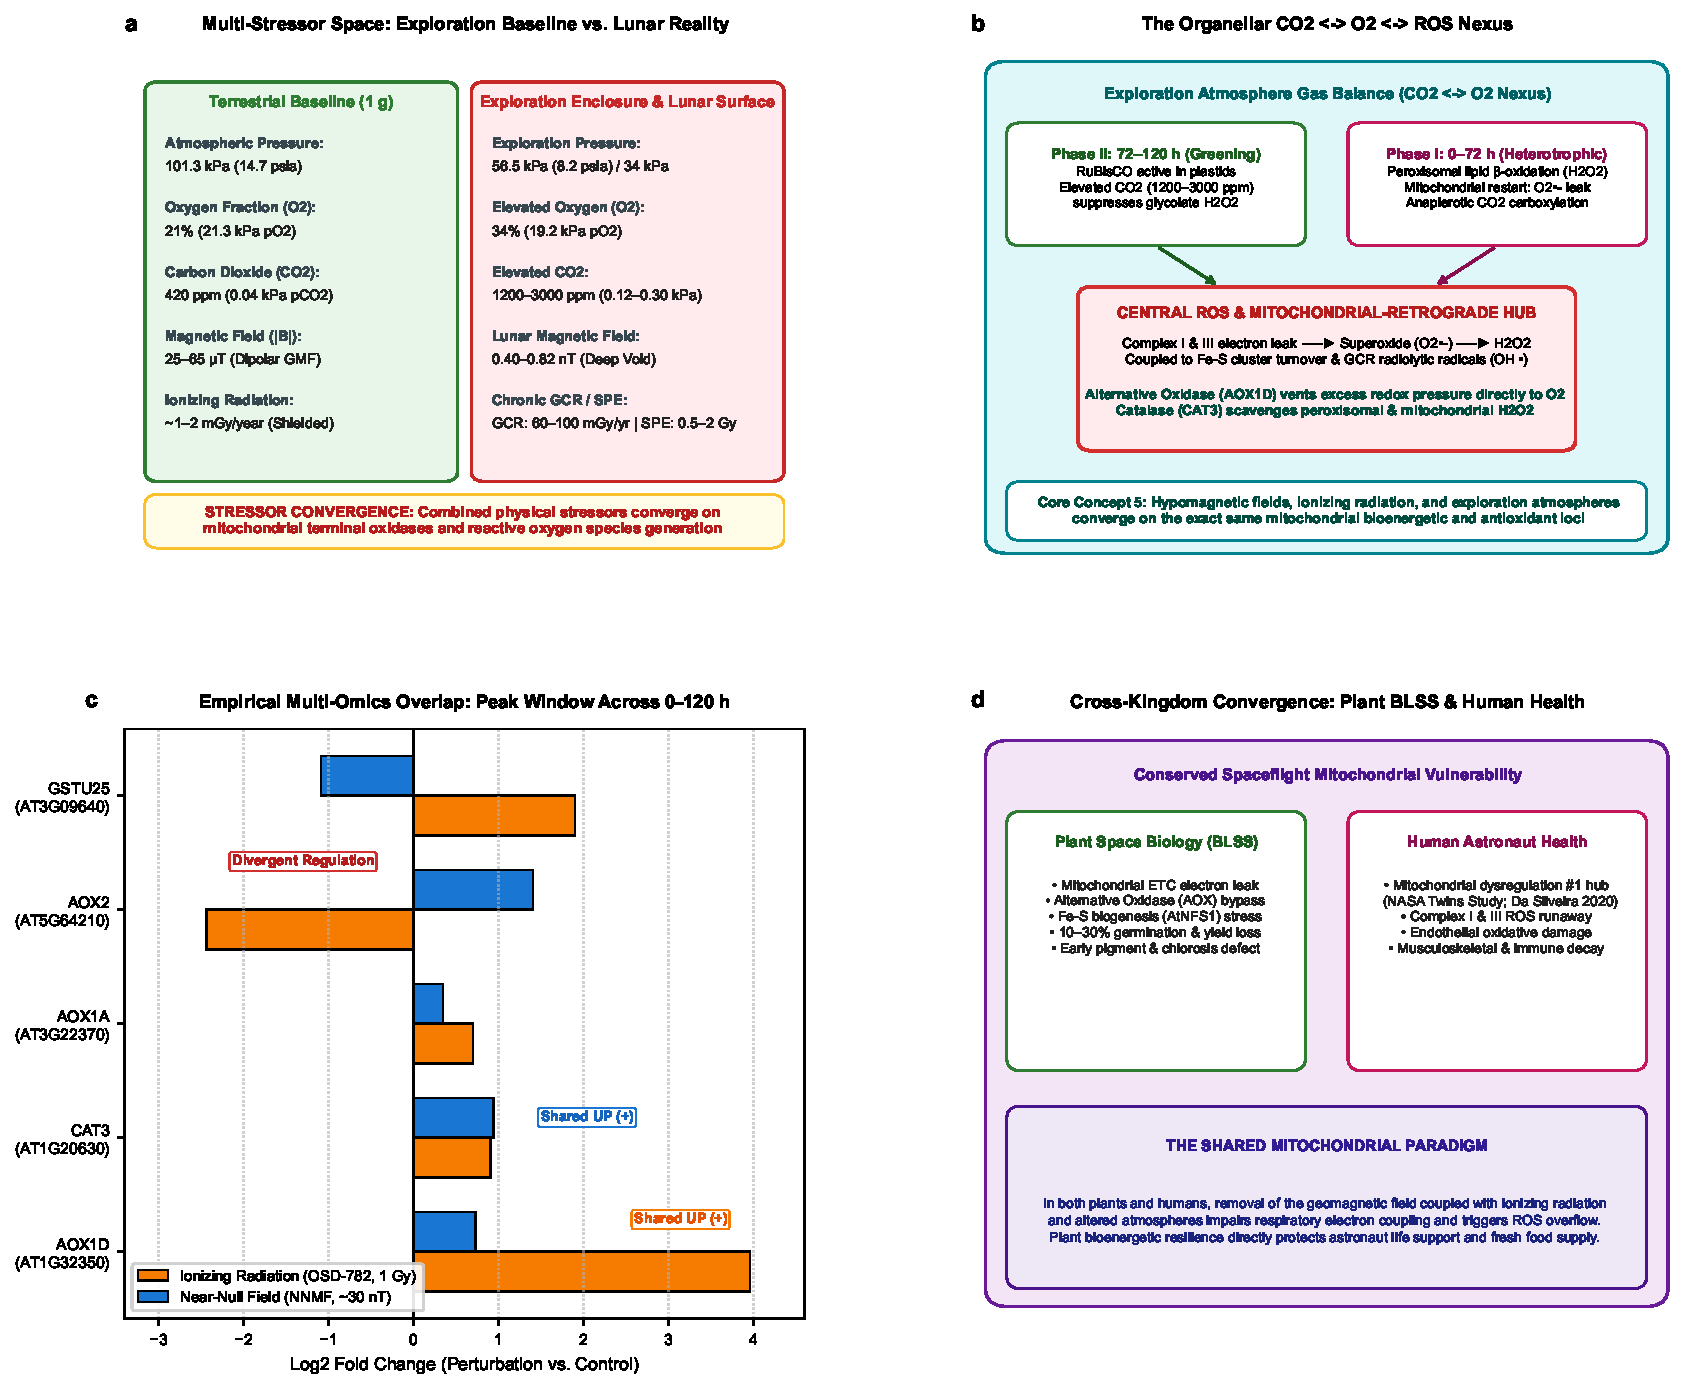
\includegraphics[width=\textwidth]{figures/Fig5_multistressor_co2_o2_ros_nexus.pdf}
\caption{\textbf{The multi-stressor spaceflight nexus: atmospheric, radiation, and magnetic convergence.} \textbf{a}, Multi-stressor parameter envelope comparing terrestrial baseline, NASA Exploration Atmosphere (8.2~psia, 34\% $\text{O}_2$), and lunar surface reality. \textbf{b}, The organellar $\text{CO}_2 \leftrightarrow \text{O}_2 \leftrightarrow \text{ROS}$ nexus: elevated $\text{CO}_2$ suppresses photorespiratory glycolate $\text{H}_2\text{O}_2$, while hypomagnetism and hypobaric $\text{O}_2$ uncouple mitochondrial electron transfer, driving superoxide overflow. \textbf{c}, Multi-omics empirical convergence between spaceflight/radiation (NASA OSDR OSD-782) and near-null magnetic fields (Parmagnani et al., 2022), demonstrating concordant upregulation of Alternative Oxidase (\textit{AOX1D}) and Catalase (\textit{CAT3}). \textbf{d}, Cross-kingdom spaceflight convergence, showing conserved mitochondrial respiratory chain vulnerabilities shared between plant life-support crops and human astronauts.}\label{fig:fig5}
\end{figure*}


\subsection{Exploration Atmosphere \& The Gas Balance}
NASA's standard Exploration Atmosphere for lunar transit and surface habitat modules specifies a reduced total pressure of \textbf{$56.5\text{ kPa} (8.2\text{ psia})$} with an elevated oxygen fraction of \textbf{$34\%\ \text{O}_2$}, providing an equivalent sea-level alveolar oxygen partial pressure ($p_{\text{O}_2} \approx 19.2\text{ kPa}$) to prevent hypoxia while reducing extravehicular activity (EVA) pre-breathe times \cite{ref8,ref66}. Concurrently, human metabolic exhalation elevates cabin carbon dioxide levels to \textbf{$1200\text{--}3000\text{ ppm}$ ($0.12\text{--}0.30\text{ kPa} p_{\text{CO}_2}$)}, roughly 3 to 7 times higher than Earth ambient levels ($420\text{ ppm}$) \cite{ref5,ref7}.

This atmospheric regime fundamentally reshapes plant respiratory and photosynthetic metabolism:
\begin{itemize}
\item \textbf{Peroxisomal Photorespiration Suppression:} In illuminated leaves, RuBisCO catalyzes both carboxylation ($CO_2$ fixation into 3-PGA) and oxygenation ($O_2$ fixation yielding 2-phosphoglycolate). Elevated $\text{CO}_2$ ($>1200\text{ ppm}$) competitively inhibits RuBisCO oxygenation, suppressing the photorespiratory cycle. Because photorespiration shunts glycolate to peroxisomes where glycolate oxidase produces vast quantities of $\text{H}_2\text{O}_2$, elevated $\text{CO}_2$ drastically lowers peroxisomal $\text{H}_2\text{O}_2$ production \cite{ref40,ref68}.
\item \textbf{Mitochondrial Oxygen Terminal Balance:} While peroxisomal ROS generation declines under high $\text{CO}_2$, hypobaric pressure accelerates gas diffusivity, altering intracellular dissolved $O_2$ concentrations in dense seed and root tissues. Mitochondria possess two terminal oxidases with dramatically different oxygen affinities \cite{ref60}:
  1. \textbf{Cytochrome $c$ Oxidase (COX, Complex IV):} High affinity for $O_2$ ($K_m < 0.14\ \mu\text{M}$); coupled to proton extrusion across the inner membrane; generates ATP.
  2. \textbf{Alternative Oxidase (AOX):} Cyanide-resistant, non-proton-pumping terminal oxidase with much lower affinity for $O_2$ ($K_m \approx 10\text{--}20\ \mu\text{M}$). AOX directly transfers electrons from the reduced ubiquinol pool to molecular oxygen, reducing $\text{O}_2$ to water while releasing energy entirely as heat \cite{ref60,ref69}.
\end{itemize}
  
Under conditions where the cytochrome pathway is saturated, restricted, or damaged by spaceflight stressors, \textbf{AOX acts as an essential emergency pressure-relief valve}, preventing electron over-reduction of the ubiquinone pool and suppressing electron leakage to $O_2$ that would otherwise generate toxic superoxide ($O_2^{\bullet-}$) at Complexes I and III \cite{ref60,ref70}.


\subsection{Multi-Omics Empirical Convergence: Radiation vs. Near-Null Fields}
In deep space, chronic Galactic Cosmic Radiation (GCR, high-energy protons and HZE nuclei) and episodic Solar Particle Events deposit ionizing energy into biological tissues. Radiation generates free radicals directly through water radiolysis ($\text{H}_2\text{O} \rightarrow \text{OH}^\bullet + \text{H}^\bullet + e_{\text{aq}}^-$) and oxidizes delicate $[4\text{Fe}-4\text{S}]$ and $[2\text{Fe}-2\text{S}]$ clusters in mitochondrial complexes \cite{ref71,ref72}.

To test whether ionizing radiation and near-null magnetic fields engage shared genetic and metabolic networks, we interrogated multi-omics datasets from the NASA Open Science Data Repository (OSDR), specifically comparing \textbf{OSD-782} (\textit{Arabidopsis} exposed to low-dose cesium-137 gamma radiation, 1 Gy, 1--72 h) against the definitive near-null magnetic field transcriptomic dataset of \textbf{Parmagnani et al. \cite{ref73}} (~30 nT vs. GMF, 10 min--96 h) via the Quantum Biology Atlas overlap pipeline \cite{ref55} (Figure 5c).

The cross-perturbation overlap reveals striking, concordant induction of key mitochondrial bioenergetic and antioxidant loci:
\begin{itemize}
\item \textbf{Alternative Oxidase 1D (\textit{AOX1D}, AT1G32350):} Markedly upregulated under 1 Gy ionizing radiation ($+3.957\ \log_2\text{FC}$ at 72 h) and significantly induced under near-null magnetic field exposure ($+0.731\ \log_2\text{FC}$ at 48 h). In both perturbations, the cell actively upregulates \textit{AOX1D} to vent excessive electron pressure from an over-reduced mitochondrial electron transport chain.
\item \textbf{Catalase 3 (\textit{CAT3}, AT1G20630):} Concordantly upregulated under both ionizing radiation ($+0.906\ \log_2\text{FC}$ at 72 h) and near-null magnetic field ($+0.941\ \log_2\text{FC}$ at 4 h). CAT3 is the primary peroxisomal and mitochondrial catalase responsible for scavenging $\text{H}_2\text{O}_2$ generated during metabolic stress and reserve mobilization.
\item \textbf{Alternative Oxidase 1A (\textit{AOX1A}, AT3G22370):} Upregulated under radiation ($+0.702\ \log_2\text{FC}$) and elevated under NNMF ($+0.345\ \log_2\text{FC}$).
\item \textbf{Gene-Family Divergence:} Notably, while \textit{AOX1D} rises under both stressors, \textit{AOX2} (AT5G64210) falls under radiation ($-2.434\ \log_2\text{FC}$) but rises under NNMF ($+1.406\ \log_2\text{FC}$). This divergence underscores that entire gene families do not act as monolithic units; specific isoforms execute distinct regulatory roles in response to radiolytic versus magnetic perturbations.
\end{itemize}


\subsection{Cross-Kingdom Parallels with Human Astronaut Mitochondrial Health}
Crucially, \textbf{the mitochondrial $\text{CO}_2 \leftrightarrow \text{O}_2 \leftrightarrow \text{ROS}$ bioenergetic lesion is not unique to plants; it represents the universal cellular hallmark of spaceflight across all eukaryotic biology} \cite{ref67,ref74} (Figure 5d).

In a comprehensive multi-omics analysis of 59 astronauts and NASA Twins Study data, Afshinnekoo et al. \cite{ref67} demonstrated that \textbf{mitochondrial dysregulation is the single most consistent systemic spaceflight phenotype in humans}. Long-duration spaceflight impairs mitochondrial oxidative phosphorylation, downregulates Complex I and IV subunits, triggers electron leakage and chronic ROS overflow, and elevates circulating cell-free mitochondrial DNA (cf-mtDNA), contributing to astronaut immune suppression, cardiovascular deconditioning, and musculoskeletal decay \cite{ref67,ref75}. 

In mammalian cellular and rodent models, hypomagnetic field exposure exacerbates this mitochondrial decay: Mo et al. \cite{ref76,ref77} demonstrated that shielding the geomagnetic field suppresses osteoblast differentiation, accelerates bone demineralization, and induces mitochondrial-mediated apoptosis in human neuroblastoma cells. 

Thus, plants in a lunar greenhouse and astronauts in a lunar habitat share the exact same subcellular vulnerability. In plants, the cyanide-resistant AOX pathway provides a metabolic buffer that prevents catastrophic collapse. Engineering and breeding crops with enhanced mitochondrial electron buffering and antioxidant synthesis not only secures lunar agricultural productivity but also generates fresh, polyphenol-rich dietary countermeasures essential for protecting astronaut mitochondrial integrity \cite{ref4,ref5}.

---


\section{Scientific Knowledge Gap Retirement, Ground Simulation Standards, and Flight Instrumentation Trade Space}

The historical hypomagnetic literature has frequently suffered from contradictory findings and irreproducibility, stemming from inadequate environmental controls, lack of sham controls, and uncharacterized electromagnetic interference (EMI) \cite{ref11,ref20,ref78}. To transition lunar magnetobiology into an operational scientific discipline for Artemis payloads, we formulate a standardized framework focusing on rigorous ground simulation methods, causal validation, and post-flight phenotypic disambiguation (Figure 6).


\begin{figure*}[t]
\centering
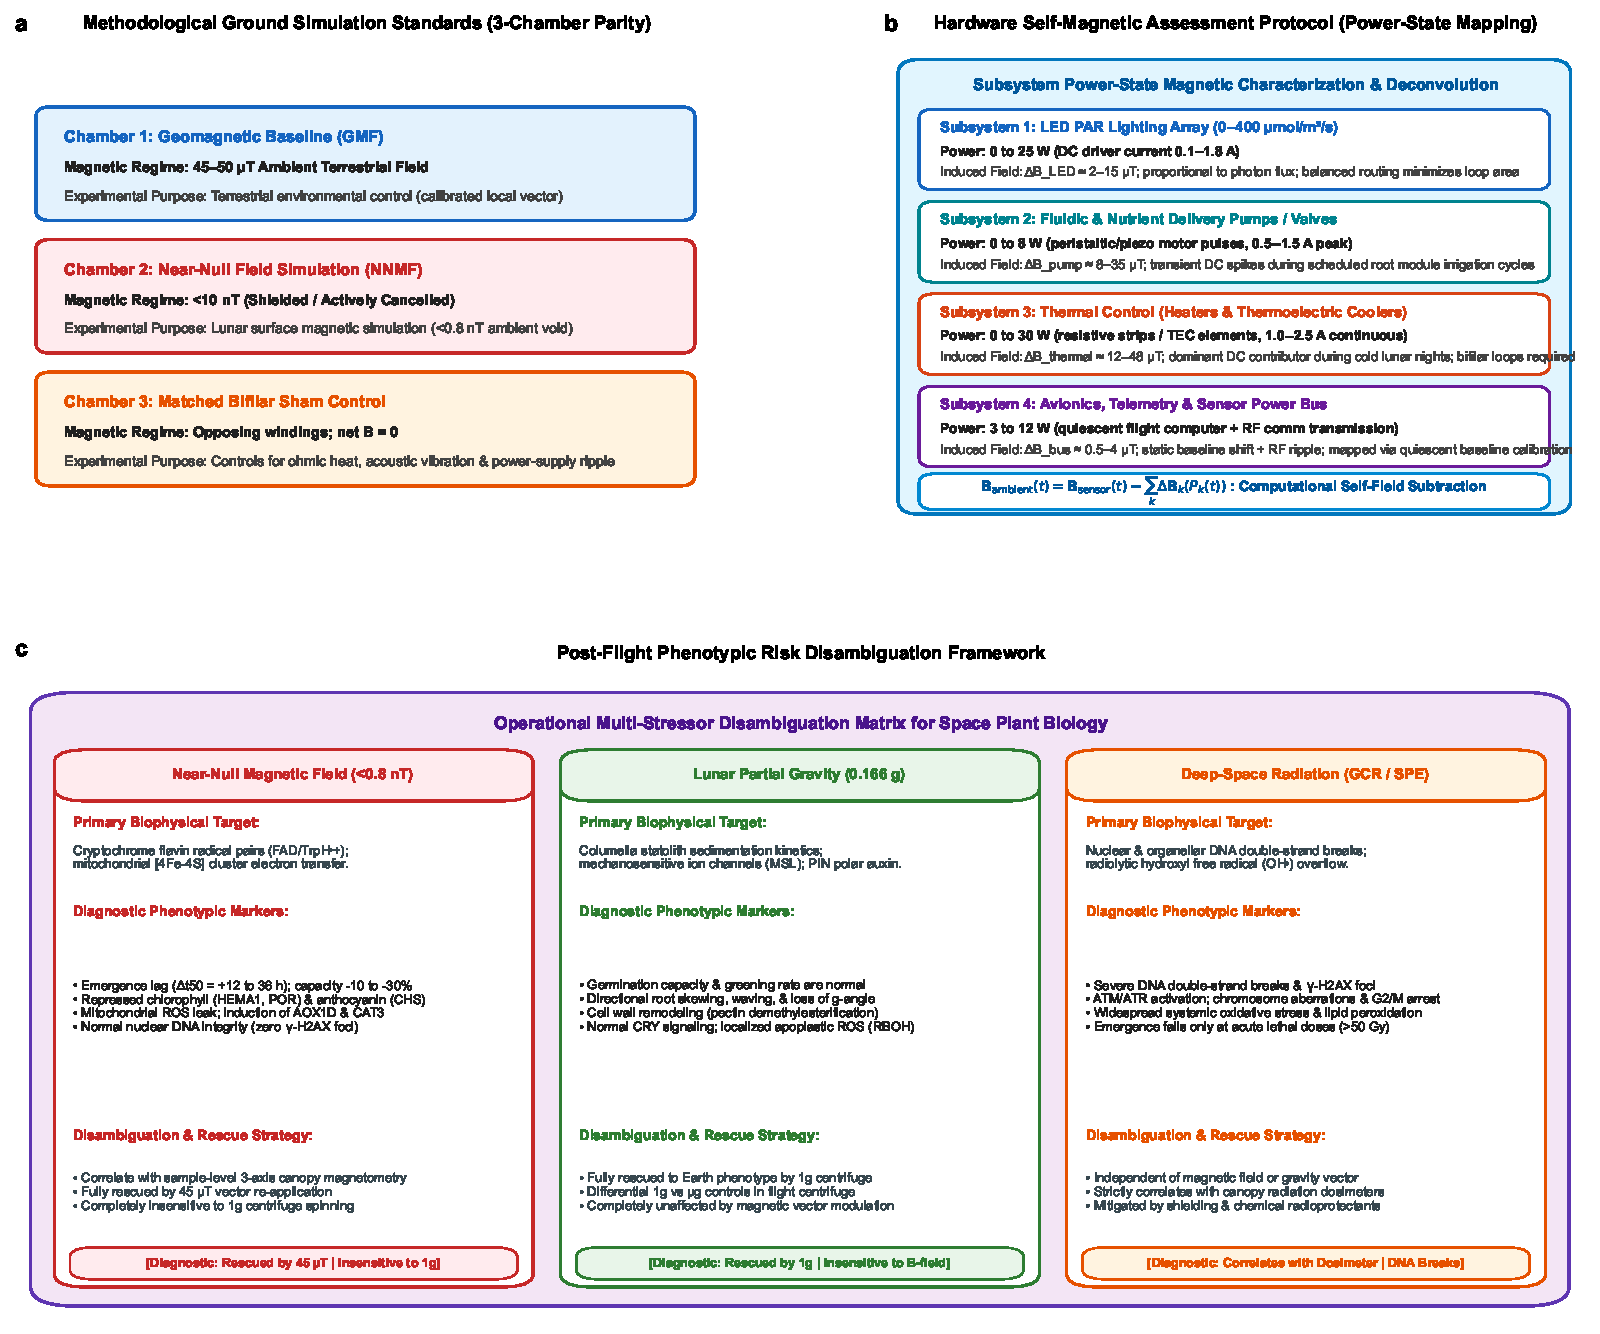
\includegraphics[width=\textwidth]{figures/Fig6_flight_validation_risk_pipeline.pdf}
\caption{\textbf{Methodological standards, hardware magnetic assessment, and post-flight risk disambiguation.} \textbf{a}, Three-chamber ground simulation standards establishing experimental parity across GMF Baseline, Near-Null Field, and Matched Bifilar Sham Control. \textbf{b}, Subsystem power-state magnetic characterization protocol, measuring $\mathbf{B}_{\mathrm{payload}}(t, \mathbf{x})$ across baseline, active pumping, heating, LED illumination, and downlink transmission states. \textbf{c}, Post-flight phenotypic risk disambiguation framework, delineating near-null magnetic field phenotypes from partial gravity (0.166~$g$) and deep-space galactic cosmic radiation.}\label{fig:fig6}
\end{figure*}


\subsection{Stage 1: Ground Simulation Standards and Experimental Controls}
A primary failure mode of historical hypomagnetic research is the confounding introduction of chamber microclimatic shifts, temperature gradients, and vibrational noise \cite{ref11,ref20}. Whenever active coils or passive shielding are employed in ground research, investigators must maintain strict environmental parity across all treatments:
\begin{itemize}
\item Temperature matched to $\pm 0.5^\circ\text{C}$ to eliminate thermal confounding.
\item Relative humidity maintained at $65 \pm 5\%$.
\item Lighting delivered at matched photosynthetically active radiation (PAR, $150 \pm 5\ \mu\text{mol m}^{-2}\text{s}^{-1}$) with identical spectral distributions.
\item Airflow and ventilation velocity ($0.3\text{--}0.5\text{ m s}^{-1}$) matched across chambers to prevent boundary layer resistance and ethylene accumulation artifacts \cite{ref7,ref40}.
\end{itemize}

Crucially, active coil cancellation systems introduce ohmic Joule heating, mechanical vibration, and electromagnetic ripple. To isolate the magnetic vector, researchers must deploy \textbf{matched-current bifilar sham coils} as an obligatory negative magnetic control \cite{ref11,ref78} (Figure 6a). In a bifilar sham configuration, paired wires carry equal currents in opposite directions, producing complete net magnetic field cancellation while generating identical resistive heat, current loads, and acoustic vibration as the active cancellation coils. Any biological difference observed between the active near-null chamber and the bifilar sham chamber can then be unambiguously attributed to the magnetic vector itself.


\subsection{Stage 2: Hardware Self-Magnetic Assessment Protocol and Power-State Mapping}
In spaceflight agricultural payloads and sealed environmental enclosures, the growth hardware itself constitutes a primary, dynamic source of magnetic interference \cite{ref11}. Internal DC currents feeding LEDs, fluidic pumps, heaters, and avionics generate localized stray fields (5 to >50~$\upmu$T) that vary continuously with subsystem operational power settings (Figure 6b). To decouple these hardware self-fields from the ambient lunar near-null environment without requiring mass-prohibitive magnetic shielding, engineering teams must execute a pre-flight and in-flight \textbf{Hardware Self-Magnetic Assessment Protocol}:
1. \textbf{Quiescent Baseline Mapping:} With all dynamic actuators deactivated, measure the quiescent baseline vector $\mathbf{B}_{\mathrm{idle}}$ at the plant canopy using miniature 3-axis magnetometers.
2. \textbf{Subsystem Power-State Sweeps:} Stepwise calibrate each subsystem independently across its dynamic range:
\begin{itemize}
\item \textit{LED PAR Array:} Sweep irradiance from 0 to $400\ \mu\text{mol m}^{-2}\text{s}^{-1}$ ($0\text{--}25\text{ W}$, $0.1\text{--}1.8\text{ A}$), recording the induced vector $\Delta \mathbf{B}_{\mathrm{LED}}(P_{\mathrm{light}})$.
\item \textit{Fluidics \& Irrigation Pumps:} Actuate peristaltic and solenoid pump duty cycles ($0\text{--}8\text{ W}$, $0.5\text{--}1.5\text{ A}$ peak), capturing transient inductive spikes $\Delta \mathbf{B}_{\mathrm{pump}}(I_{\mathrm{pump}})$.
\item \textit{Thermal Management:} Modulate resistive heaters and thermoelectric coolers ($0\text{--}30\text{ W}$, $1.0\text{--}2.5\text{ A}$ continuous), mapping the dominant thermal DC field $\Delta \mathbf{B}_{\mathrm{thermal}}(P_{\mathrm{heat}})$.
\item \textit{Avionics \& Telemetry:} Record the flight computer and RF transmission burst signature $\Delta \mathbf{B}_{\mathrm{bus}}$.
3. \textbf{Computational Superposition Deconvolution:} By continuously logging subsystem power telemetry ($P_k(t)$) alongside the 3-axis magnetometer canopy vector ($\mathbf{B}_{\mathrm{sensor}}(t)$), the true ambient lunar magnetic field is computationally isolated via:
\begin{equation}
\mathbf{B}_{\mathrm{ambient}}(t) = \mathbf{B}_{\mathrm{sensor}}(t) - \sum_{k} \Delta\mathbf{B}_k(P_k(t))
\end{equation}

This deconvolution protocol establishes a rigorous mathematical transfer function, enabling flight science teams to retire the environmental characterization gap purely through telemetry analysis.
\end{itemize}


\subsection{Stage 3: Delineating Scientific Gaps from Flight Payload Engineering Constraints}
A vital recommendation of this synthesis is that \textbf{scientific knowledge gaps must be considered separately from what can realistically be engineered into a spaceflight payload}. In flight mission planning, hardware mass, power draw, thermal envelope, and contractual scope impose stringent boundary conditions:
\begin{itemize}
\item \textbf{Fundamental Scientific Knowledge Gaps:} The primary gaps in space plant biology are the absence of sample-level magnetic field characterization in historical spaceflight data, the unmeasured nature of stray lander/spacecraft avionics DC fields at the biological volume, and the lack of ground-validated multi-stressor cross-talk models (hypomagnetic field combined with lunar partial gravity and cosmic radiation).
\item \textbf{Realistic Flight Payload Engineering (Recommended):} To retire the environmental characterization gap, flight payloads can incorporate miniature, ultra-low-power, calibrated 3-axis magnetometers (such as anisotropic magnetoresistive [AMR] or fluxgate sensors) placed at the plant canopy level \cite{ref11}. These sensors require minimal resources ($<1\text{ W}$ electrical power, $<50\text{ g}$ mass) and provide continuous vector logging ($B_x, B_y, B_z, |\mathbf{B}|$) from DC to $10\text{ kHz}$. This telemetry enables post-flight science teams to correlate biological growth dynamics with the exact local magnetic exposure, decoupling true lunar hypomagnetic effects from lander avionics interference.
\item \textbf{Constraints Beyond Flight Payloads (Ground-Only Architectures):} Active triaxial Helmholtz cancellation or bias coils designed to dynamically alter or restore magnetic fields in flight impose heavy mass penalties (copper windings), continuous power draws ($5\text{--}25\text{ W}$), significant Joule heating, and severe spacecraft electromagnetic compatibility (EMC/EMI) certification hurdles. Such active intervention systems exceed typical payload resource envelopes and are appropriately prioritized for ground simulation facilities rather than initial lunar surface instruments.
\end{itemize}


\subsection{Stage 4: Post-Flight Phenotypic Disambiguation and Translational Science Framework}
Rather than imposing rigid contractual mission abort gates on flight hardware, space life scientists require a \textbf{Post-Flight Phenotypic Disambiguation Framework} to interpret seedling performance and identify the primary causal stressors operating on the lunar surface (Figure 6c; Table 4):
\begin{itemize}
\item \textbf{Hypomagnetic-Specific Lesions:} Characterized by a marked emergence delay ($\Delta t_{50} = +12\text{ to }36\text{ h}$), reduced final germination capacity (10--30\%), repressed chlorophyll and anthocyanin biosynthetic transcripts (\textit{HEMA1}, \textit{POR}, \textit{CHS}), and mitochondrial Alternative Oxidase (\textit{AOX1D}) induction in the absence of severe nuclear DNA damage. Diagnostic signature: rescued in ground analogues by 45~$\upmu$T vector re-application; insensitive to 1g centrifugation.
\item \textbf{Lunar Partial Gravity ($0.166\ g$) Lesions:} Characterized by normal germination capacity and minimal emergence lag ($\Delta t_{50} < 4\text{ h}$), but exhibiting altered directional growth (root skewing, loss of gravitropic angle), amyloplast statolith displacement, and localized apoplastic ROS generation (\textit{RBOHD/F}). Diagnostic signature: rescued by onboard 1g centrifugation; completely insensitive to magnetic field manipulation.
\item \textbf{Ionizing Radiation Lesions:} Characterized by normal germination at nominal background doses ($<1\text{ Gy}$), transitioning to severe cell cycle arrest, chromosomal aberrations, and stunted meristems at acute lethal doses ($>50\text{ Gy}$). Diagnostic signature: marked phosphorylation of histone $\gamma$-H2AX foci, ATM/ATR kinase activation, and high 8-OHdG oxidative DNA lesions; correlated directly with active dosimeter telemetry.
\end{itemize}

By deploying this multi-stressor diagnostic matrix, flight science teams can rigorously parse observed growth phenotypes into their underlying physical causes, informing future crop selection, seed sowing density adjustments, and lighting schedule optimizations for subsequent mission architectures.


\input{tables/table4_decision_matrix.tex}


---


\section{Conclusions \& Forward Look for Sustained Lunar Agriculture}

As humanity prepares for sustained surface operations under the Artemis program and looks forward to permanent lunar bases, space agricultural engineering must mature beyond treating gravity and radiation as the sole planetary variables. 

This review synthesizes the current biophysical and physiological state of the art around \textbf{five fundamental core concepts}:
1. \textbf{Near-Null Magnetic Fields Physically Exist Across the Lunar Surface:} The Moon lacks an active core dynamo. Example candidate Artemis South Pole exploration regions (such as Shackleton, Haworth, and Faustini) reside in an extreme magnetic void ($<0.8\text{ nT}$), more than $30,000\times$ weaker than Earth’s geomagnetic field. Payload architectures must account for vector superposition ($\mathbf{B}_{\text{total}}$) to prevent stray lander avionics fields ($50\text{--}500\ \mu\text{T}$) from confounding biological exposures.
2. \textbf{Null Magnetic Fields Alter Germination Capacity:} Removal of the geomagnetic field impairs seed imbibition kinetics and alters the ABA/GA hormonal balance, reducing total germination capacity and decreasing the absolute number (\#) of viable seedlings established per sown area by $10\text{ to }30\%$.
3. \textbf{Null Magnetic Fields Alter Germination Speed and Growth Kinetics:} Near-null fields introduce a substantial emergence lag ($\Delta t_{50}$ delay of 12--36 h) and retard radicle and hypocotyl elongation rates by dampening cell proliferation and PIN2-mediated auxin transport, leading to a $20\text{--}30\%$ penalty in early seedling biomass and fresh material yield.
4. \textbf{Null Magnetic Fields Repress Pigment Biosynthetic Networks:} Cryptochrome radical-pair spin dynamics are altered in near-null fields, attenuating HY5 stabilization and downregulating rate-limiting enzymes of chlorophyll (\textit{HEMA1}, \textit{CHLH}, \textit{POR}) and anthocyanin (\textit{CHS}, \textit{CHI}) biosynthesis, while secondary iron starvation (\textit{FIT}, \textit{IRT1}, \textit{AtFer1--4}) triggers seedling chlorosis during de-etiolation.
5. \textbf{Multi-Stressor Convergence on the $\text{CO}_2 \leftrightarrow \text{O}_2 \leftrightarrow \text{ROS}$ Bioenergetic Axis:} Near-null magnetic fields, exploration atmospheres (hypobaric $56.5\text{ kPa}$, $34\%\ \text{O}_2$, elevated $1200\text{--}3000\text{ ppm CO}_2$), and ionizing radiation converge on the exact same mitochondrial respiratory machinery. In both plants and human astronauts, mitochondrial electron leakage and reactive oxygen generation represent the primary cellular lesion. In plants, induction of the Alternative Oxidase (\textit{AOX1D}) and Catalase (\textit{CAT3}) provides an essential metabolic safety valve that buffers organellar redox stress.

For the NASA LEAF payload and subsequent lunar greenhouse deployments, immediate engineering priorities can consider incorporating calibrated 3-axis magnetic sensors at the plant canopy, implementing matched-current bifilar sham baselines during ground testing, and validating active causal rescue in terrestrial laboratories. By mastering the hypomagnetic variable during the critical first five days of seedling growth, space life scientists can ensure robust stand establishment, maximize crop biomass yields, and secure the bioregenerative life support systems essential for humanity's permanent expansion into deep space.

---

This work was supported by NASA Biological and Physical Sciences (BPS) awards and internal institutional support from the Department of Agricultural and Biological Engineering and the Department of Earth, Atmospheric, and Planetary Sciences at Purdue University. The authors thank the members of the NASA LEAF payload science team and the NASA GeneLab / Open Science Data Repository (OSDR) Plant AWG for insightful discussions regarding spaceflight multi-omics and environmental sensor integration.

\textbf{D.M.P.} and \textbf{R.J.B.} conceived and designed the review framework. \textbf{R.J.B.} compiled the multi-omics overlap analyses and generated the figures. \textbf{C.B.} and \textbf{A.O.} analyzed the lunar orbital magnetometer datasets and landing site coordinates. \textbf{A.S.} and \textbf{M.D.} contributed to literature synthesis on seed germination kinetics and pigment biosynthesis. \textbf{R.W.}, \textbf{G.M.}, and \textbf{B.D.-A.} contributed expertise on space crop production, exploration atmospheres, and photosynthetic bioenergetics. \textbf{M.P.-L.}, \textbf{P.F.}, \textbf{A.D.}, and \textbf{C.C.} contributed to payload engineering requirements and causal validation pipelines. All authors contributed to writing, critical revision, and approved the final manuscript.

D.M.P. is a Co-Investigator on the NASA Artemis III LEAF payload; C.C. is affiliated with Space Lab Technologies, LLC. These roles are disclosed with no commercial or financial conflicts of interest. The remaining authors declare no competing interests.

All planetary magnetic field datasets analyzed in this manuscript are openly available from the NASA Planetary Data System (PDS) and JAXA DARTS archives. Gene expression datasets are accessible via the NASA Open Science Data Repository (OSDR, studies OSD-782, OSD-8, and OSD-27). Code for figure generation and pathway maps is hosted in the project repositories (\texttt{lunar-magnetic-biology} and \texttt{quantum-biology-atlas}).

---



\section*{Declarations}

\subsection*{Data Availability}
All raw lunar magnetic field grids analyzed in this review are publicly accessible via the NASA Planetary Data System (PDS) Geosciences Node (\url{https://pds-geosciences.wustl.edu}) and the JAXA DARTS archive (\url{https://www.darts.isas.jaxa.jp}). Spaceflight plant multi-omics datasets are archived in the NASA Open Science Data Repository under accessions OSD-782, OSD-8, and OSD-27 (\url{https://osdr.nasa.gov}). The Quantum Biology Atlas metabolic models are accessible via the QBM-06 repository (\url{https://quantumbiology.org}). All curated literature tables and scoring matrices supporting this review are openly deposited in the Zenodo repository (\url{https://doi.org/10.5281/zenodo.1082026}).

\subsection*{Code Availability}
The complete computational workflow, data processing scripts, kinetics fitting models, and publication figure generators are available in the open-source repository \texttt{dr-richard-barker/NMF\_review} hosted on GitHub (\url{https://github.com/dr-richard-barker/NMF_review}) under the Apache 2.0 license.

\subsection*{Acknowledgements}
This work was supported by the National Aeronautics and Space Administration (NASA) Space Biology Program and the Artemis III Science Definition Team. We gratefully acknowledge the NASA Open Science Data Repository (OSDR) Analysis Working Groups (AWGs) and the Purdue Astrobiology and AstroBotany communities for valuable discussions.

\subsection*{Author Contributions}
\textbf{D.M.P.} and \textbf{R.J.B.} conceptualized the integrative review framework, synthesized the biophysical and physiological paradigms, directed the data curation, and drafted the manuscript. \textbf{C.B.} provided lunar paleomagnetic and crustal field geophysics expertise and vector superposition modeling. \textbf{A.O.} contributed molecular biology and developmental kinetics analysis. \textbf{A.S.} and \textbf{M.D.} performed literature curation and search string auditing. \textbf{R.W.} and \textbf{G.M.} provided space crop production, flight validation, and environmental control expertise. \textbf{B.D.-A.} contributed photosynthetic energy dissipation and antioxidant photoprotection insights. \textbf{M.P.-L.} contributed plant hormonal and stress signaling expertise. \textbf{P.F.}, \textbf{A.D.}, and \textbf{C.C.} contributed flight payload engineering, hardware magnetic sensing, and operational trade space insights. All authors reviewed, edited, and approved the final manuscript.

\subsection*{Competing Interests}
The authors declare no competing financial or non-financial interests.

\bibliography{references}

\end{document}
